% Options for packages loaded elsewhere
\PassOptionsToPackage{unicode}{hyperref}
\PassOptionsToPackage{hyphens}{url}
\PassOptionsToPackage{dvipsnames,svgnames,x11names}{xcolor}
%
\documentclass[
  11pt,
]{article}

\usepackage{amsmath,amssymb}
\usepackage{setspace}
\usepackage{iftex}
\ifPDFTeX
  \usepackage[T1]{fontenc}
  \usepackage[utf8]{inputenc}
  \usepackage{textcomp} % provide euro and other symbols
\else % if luatex or xetex
  \usepackage{unicode-math}
  \defaultfontfeatures{Scale=MatchLowercase}
  \defaultfontfeatures[\rmfamily]{Ligatures=TeX,Scale=1}
\fi
\usepackage{lmodern}
\ifPDFTeX\else  
    % xetex/luatex font selection
\fi
% Use upquote if available, for straight quotes in verbatim environments
\IfFileExists{upquote.sty}{\usepackage{upquote}}{}
\IfFileExists{microtype.sty}{% use microtype if available
  \usepackage[]{microtype}
  \UseMicrotypeSet[protrusion]{basicmath} % disable protrusion for tt fonts
}{}
\makeatletter
\@ifundefined{KOMAClassName}{% if non-KOMA class
  \IfFileExists{parskip.sty}{%
    \usepackage{parskip}
  }{% else
    \setlength{\parindent}{0pt}
    \setlength{\parskip}{6pt plus 2pt minus 1pt}}
}{% if KOMA class
  \KOMAoptions{parskip=half}}
\makeatother
\usepackage{xcolor}
\usepackage[margin=1in]{geometry}
\setlength{\emergencystretch}{3em} % prevent overfull lines
\setcounter{secnumdepth}{5}
% Make \paragraph and \subparagraph free-standing
\ifx\paragraph\undefined\else
  \let\oldparagraph\paragraph
  \renewcommand{\paragraph}[1]{\oldparagraph{#1}\mbox{}}
\fi
\ifx\subparagraph\undefined\else
  \let\oldsubparagraph\subparagraph
  \renewcommand{\subparagraph}[1]{\oldsubparagraph{#1}\mbox{}}
\fi


\providecommand{\tightlist}{%
  \setlength{\itemsep}{0pt}\setlength{\parskip}{0pt}}\usepackage{longtable,booktabs,array}
\usepackage{calc} % for calculating minipage widths
% Correct order of tables after \paragraph or \subparagraph
\usepackage{etoolbox}
\makeatletter
\patchcmd\longtable{\par}{\if@noskipsec\mbox{}\fi\par}{}{}
\makeatother
% Allow footnotes in longtable head/foot
\IfFileExists{footnotehyper.sty}{\usepackage{footnotehyper}}{\usepackage{footnote}}
\makesavenoteenv{longtable}
\usepackage{graphicx}
\makeatletter
\def\maxwidth{\ifdim\Gin@nat@width>\linewidth\linewidth\else\Gin@nat@width\fi}
\def\maxheight{\ifdim\Gin@nat@height>\textheight\textheight\else\Gin@nat@height\fi}
\makeatother
% Scale images if necessary, so that they will not overflow the page
% margins by default, and it is still possible to overwrite the defaults
% using explicit options in \includegraphics[width, height, ...]{}
\setkeys{Gin}{width=\maxwidth,height=\maxheight,keepaspectratio}
% Set default figure placement to htbp
\makeatletter
\def\fps@figure{htbp}
\makeatother

\usepackage{booktabs}
\usepackage{longtable}
\usepackage{array}
\usepackage{multirow}
\usepackage{wrapfig}
\usepackage{float}
\usepackage{colortbl}
\usepackage{pdflscape}
\usepackage{tabu}
\usepackage{threeparttable}
\usepackage{threeparttablex}
\usepackage[normalem]{ulem}
\usepackage{makecell}
\usepackage{xcolor}
\usepackage{amsmath}
\usepackage{amssymb}
\usepackage{booktabs}
\usepackage{float}
\usepackage{longtable}
\usepackage{graphicx}
\usepackage{caption}
\makeatletter
\@ifpackageloaded{caption}{}{\usepackage{caption}}
\AtBeginDocument{%
\ifdefined\contentsname
  \renewcommand*\contentsname{Table of contents}
\else
  \newcommand\contentsname{Table of contents}
\fi
\ifdefined\listfigurename
  \renewcommand*\listfigurename{List of Figures}
\else
  \newcommand\listfigurename{List of Figures}
\fi
\ifdefined\listtablename
  \renewcommand*\listtablename{List of Tables}
\else
  \newcommand\listtablename{List of Tables}
\fi
\ifdefined\figurename
  \renewcommand*\figurename{Figure}
\else
  \newcommand\figurename{Figure}
\fi
\ifdefined\tablename
  \renewcommand*\tablename{Table}
\else
  \newcommand\tablename{Table}
\fi
}
\@ifpackageloaded{float}{}{\usepackage{float}}
\floatstyle{ruled}
\@ifundefined{c@chapter}{\newfloat{codelisting}{h}{lop}}{\newfloat{codelisting}{h}{lop}[chapter]}
\floatname{codelisting}{Listing}
\newcommand*\listoflistings{\listof{codelisting}{List of Listings}}
\makeatother
\makeatletter
\makeatother
\makeatletter
\@ifpackageloaded{caption}{}{\usepackage{caption}}
\@ifpackageloaded{subcaption}{}{\usepackage{subcaption}}
\makeatother
\ifLuaTeX
  \usepackage{selnolig}  % disable illegal ligatures
\fi
\usepackage{bookmark}

\IfFileExists{xurl.sty}{\usepackage{xurl}}{} % add URL line breaks if available
\urlstyle{same} % disable monospaced font for URLs
\hypersetup{
  pdftitle={Identifying Variation, Facility Size, and Capacity in the UST Replacement Model},
  pdfauthor={Kaleb Javier},
  colorlinks=true,
  linkcolor={blue},
  filecolor={Maroon},
  citecolor={Blue},
  urlcolor={Blue},
  pdfcreator={LaTeX via pandoc}}

\title{Identifying Variation, Facility Size, and Capacity in the UST
Replacement Model}
\usepackage{etoolbox}
\makeatletter
\providecommand{\subtitle}[1]{% add subtitle to \maketitle
  \apptocmd{\@title}{\par {\large #1 \par}}{}{}
}
\makeatother
\subtitle{Diagnostic report on what the structural model uses and what
it currently ignores}
\author{Kaleb Javier}
\date{2026-06-01}

\begin{document}
\maketitle

\renewcommand*\contentsname{Table of contents}
{
\hypersetup{linkcolor=}
\setcounter{tocdepth}{3}
\tableofcontents
}
\setstretch{1.15}
\section{Setup}\label{setup}

This report documents four things:

\begin{enumerate}
\def\labelenumi{\arabic{enumi}.}
\tightlist
\item
  \textbf{Where the dynamic replacement model gets its identifying
  variation} --- visualizing the cross-cell joint distribution of
  premium \(P\) and hazard \(h\), the time-series shifts in \(P\), and
  the empirical action heterogeneity.
\item
  \textbf{The size dimension (\texttt{n\_tanks\_active})} --- empirical
  evidence that facility size, currently averaged away by the model, is
  a meaningful driver of action probabilities.
\item
  \textbf{The capacity dimension (\texttt{total\_capacity})} ---
  analogous evidence for total tank capacity in gallons, distinct from
  tank count.
\item
  \textbf{Facility-portfolio behavior around closure events}
  (Section~\ref{sec-closure-taxonomy}) --- what does a tank closure
  actually mean for the facility? Classifying every closure event by the
  facility's subsequent install behavior, and mapping those
  facility-level realities to current and proposed model actions.
\end{enumerate}

Sample throughout: the canonical observed DCM panel (TX 2006+, controls
1999+; \(N = 2{,}282{,}735\) facility-year observations across 139,493
unique facilities). The fit referenced for model-implied quantities is
the 6-parameter universal-\(\gamma\) stayFE-profile specification with
SD and MO dropped
(\texttt{Model\_Replacement\_6paramFE\_profile\_observed\_dropSDMO.rds}
from Ticket 005).

The takeaway upfront: \textbf{the joint \((P, h)\) variation cleanly
identifies the universal-\(\gamma\) structural parameters}, but
\textbf{facility size and capacity capture systematic behavioral
heterogeneity that the current 32-state model averages away}, and
\textbf{the model's action definitions (Exit vs Replace vs Maintain)
conflate genuinely different facility-portfolio behaviors}. Section 4
quantifies the action-definition issue: how much of the current ``Exit''
data is actually a partial-shrinkage event where the facility kept
operating, and how much is a true facility-level walk-away.

\section{Identifying variation in the structural
model}\label{identifying-variation-in-the-structural-model}

\subsection{\texorpdfstring{Premium \(\times\) hazard cell-level
scatter}{Premium \textbackslash times hazard cell-level scatter}}\label{sec-Ph-scatter}

The structural identification of
\((\gamma_{\text{price}}, \gamma_{\text{risk}})\) requires that \(P\)
and \(h\) vary \emph{independently} across some subset of the data.
Figure~\ref{fig-Ph-scatter} plots the 32 state cells of the model in
\((P, h)\) space, colored by regime. \textbf{Under FF}, \(P\) is set
administratively and is uncorrelated with \(h\) within the regime ---
that is the source of clean \(\gamma_{\text{price}}\) identification.
\textbf{Under RB}, \(P\) is risk-priced (covaries with \(h\)); the RB
cells provide fit but cannot separately identify
\(\gamma_{\text{price}}\) from \(\gamma_{\text{risk}}\).

\begin{figure}[H]

\caption{\label{fig-Ph-scatter}Cell-level joint distribution of annual
premium and hazard probability across the 32 state cells of the
structural model. Each point is one (age \(\times\) wall \(\times\)
regime) cell. FF cells span a range of hazards at roughly constant
premium; RB cells show premium covarying with hazard.}

\centering{

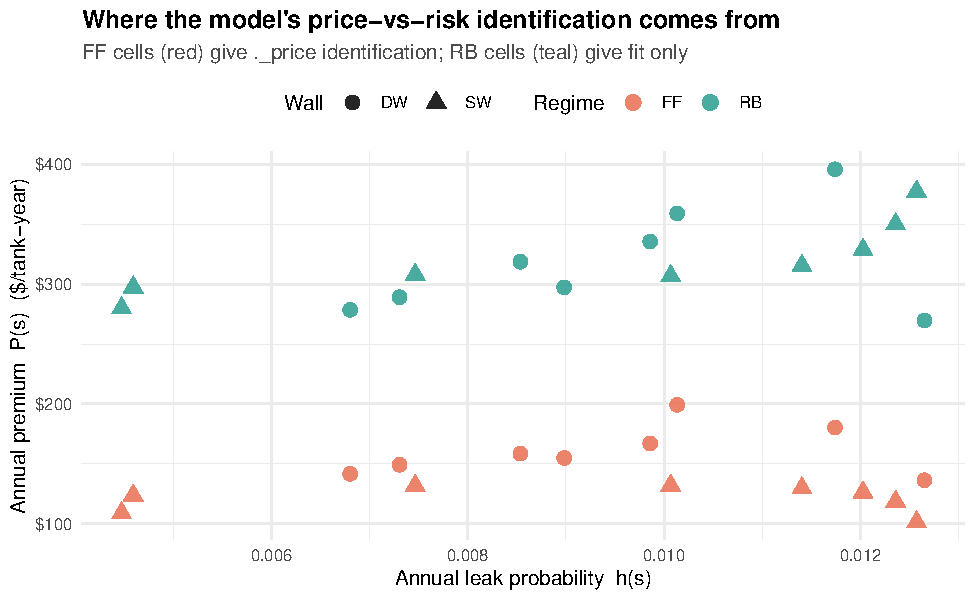
\includegraphics{Identifying_Variation_Size_Capacity_files/figure-pdf/fig-Ph-scatter-1.pdf}

}

\end{figure}%

\subsection{Cross-state, cross-year premium variation within
FF}\label{cross-state-cross-year-premium-variation-within-ff}

Within the FF regime, premium variation across states and over time
provides additional identifying power for \(\gamma_{\text{price}}\).
Figure~\ref{fig-P-time} shows year-by-year mean premium by regime in the
DCM sample. The pre-2006 TX (extended sample, included for context) had
a different premium structure than post-2006; control-state FF premiums
also drift over the sample window.

\begin{figure}[H]

\caption{\label{fig-P-time}Mean annual premium per tank by regime and
year. TX shows the FF-to-RB transition at the 2006 reform; control
states have continuous FF premium drift.}

\centering{

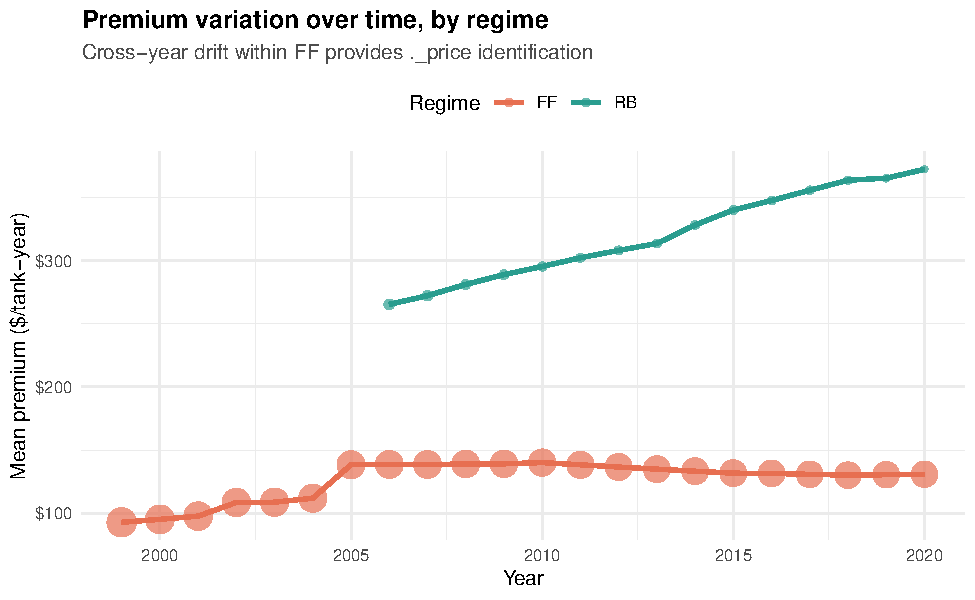
\includegraphics{Identifying_Variation_Size_Capacity_files/figure-pdf/fig-P-time-1.pdf}

}

\end{figure}%

\subsection{Empirical action shares across the 32 state
cells}\label{sec-emp-ccp}

Table~\ref{tbl-emp-ccp} summarizes the empirical action shares across
the 32 cells. This is the variation the structural likelihood is trying
to fit; the fit figures in \texttt{Dynamic\_Model\_Fit\_Report.qmd} show
the model-implied overlay.

\begingroup\fontsize{7}{9}\selectfont

\begin{longtable}{rllrrrrrrr}

\caption{\label{tbl-emp-ccp}Empirical action shares by (wall \(\times\)
regime \(\times\) age bin) cell, with cell sample size \(n\) and dollar
premium / hazard-loss values.}

\tabularnewline

\toprule
Cell & Wall & Reg & Age & N obs & Premium USD per yr & Haz loss USD per yr & Maintain pct & Exit pct & Replace pct\\
\midrule
\endfirsthead
\multicolumn{10}{@{}l}{\textit{(continued)}}\\
\toprule
Cell & Wall & Reg & Age & N obs & Premium USD per yr & Haz loss USD per yr & Maintain pct & Exit pct & Replace pct\\
\midrule
\endhead

\endfoot
\bottomrule
\endlastfoot
1 & SW & FF & 1 & 46,709 & 109 & 2925 & 98.33 & 1.46 & 0.201\\
2 & SW & FF & 2 & 97,999 & 124 & 2991 & 98.52 & 1.13 & 0.350\\
3 & SW & FF & 3 & 180,163 & 132 & 3602 & 97.49 & 2.17 & 0.340\\
4 & SW & FF & 4 & 240,344 & 132 & 4784 & 97.15 & 2.58 & 0.271\\
5 & SW & FF & 5 & 255,278 & 130 & 5307 & 97.19 & 2.63 & 0.174\\
\addlinespace
6 & SW & FF & 6 & 234,030 & 126 & 4954 & 97.69 & 2.20 & 0.113\\
7 & SW & FF & 7 & 191,377 & 118 & 4351 & 97.95 & 1.95 & 0.092\\
8 & SW & FF & 8 & 410,728 & 101 & 3780 & 98.52 & 1.45 & 0.032\\
9 & DW & FF & 1 & 64,621 & 136 & 4992 & 99.90 & 0.00 & 0.099\\
10 & DW & FF & 2 & 77,103 & 142 & 2280 & 99.36 & 0.00 & 0.636\\
\addlinespace
11 & DW & FF & 3 & 77,966 & 149 & 1948 & 99.08 & 0.00 & 0.920\\
12 & DW & FF & 4 & 62,241 & 155 & 2043 & 98.93 & 0.00 & 1.067\\
13 & DW & FF & 5 & 41,520 & 159 & 1454 & 99.31 & 0.00 & 0.686\\
14 & DW & FF & 6 & 20,407 & 167 & 1502 & 99.74 & 0.00 & 0.265\\
15 & DW & FF & 7 & 4,872 & 199 & 2165 & 99.47 & 0.00 & 0.534\\
\addlinespace
16 & DW & FF & 8 & 2,867 & 180 & 3733 & 99.62 & 0.00 & 0.384\\
17 & SW & RB & 1 & 3,350 & 280 & 2925 & 99.37 & 0.54 & 0.090\\
18 & SW & RB & 2 & 9,999 & 297 & 2991 & 98.81 & 1.12 & 0.070\\
19 & SW & RB & 3 & 19,093 & 308 & 3602 & 98.73 & 1.04 & 0.225\\
20 & SW & RB & 4 & 26,212 & 307 & 4784 & 97.75 & 2.06 & 0.198\\
\addlinespace
21 & SW & RB & 5 & 36,841 & 315 & 5307 & 97.27 & 2.58 & 0.149\\
22 & SW & RB & 6 & 37,789 & 328 & 4954 & 97.32 & 2.48 & 0.198\\
23 & SW & RB & 7 & 31,888 & 350 & 4351 & 96.85 & 2.92 & 0.223\\
24 & SW & RB & 8 & 30,722 & 377 & 3780 & 95.79 & 4.01 & 0.205\\
25 & DW & RB & 1 & 18,813 & 270 & 4992 & 99.95 & 0.00 & 0.053\\
\addlinespace
26 & DW & RB & 2 & 16,557 & 278 & 2280 & 99.43 & 0.00 & 0.568\\
27 & DW & RB & 3 & 14,499 & 289 & 1948 & 99.26 & 0.00 & 0.738\\
28 & DW & RB & 4 & 13,106 & 297 & 2043 & 98.02 & 0.00 & 1.976\\
29 & DW & RB & 5 & 8,677 & 319 & 1454 & 97.49 & 0.00 & 2.512\\
30 & DW & RB & 6 & 4,218 & 335 & 1502 & 98.29 & 0.00 & 1.707\\
\addlinespace
31 & DW & RB & 7 & 1,770 & 359 & 2165 & 98.08 & 0.00 & 1.921\\
32 & DW & RB & 8 & 976 & 396 & 3733 & 98.16 & 0.00 & 1.844\\*

\end{longtable}

\endgroup{}

\section{The size dimension: number of tanks per
facility}\label{the-size-dimension-number-of-tanks-per-facility}

\subsection{Distribution}\label{distribution}

The DCM sample has substantial spread in facility size. Only
\textbf{23\%} of facility-years are single-tank; the median
facility-year has \textbf{3 tanks}; 24\% have \textbf{4 or more}.

\begin{figure}[H]

\caption{\label{fig-size-dist}Distribution of active tank count per
facility-year in the DCM observed sample. Bars truncated at 8+; about
1.6\% of facility-years have \(\geq 8\) tanks.}

\centering{

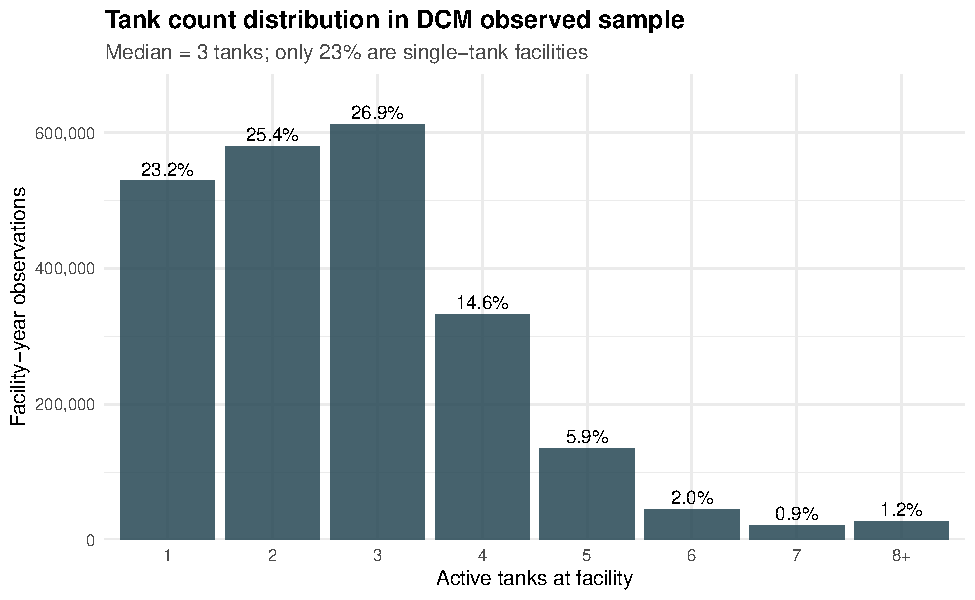
\includegraphics{Identifying_Variation_Size_Capacity_files/figure-pdf/fig-size-dist-1.pdf}

}

\end{figure}%

\subsection{\texorpdfstring{Action shares by (size \(\times\)
wall)}{Action shares by (size \textbackslash times wall)}}\label{action-shares-by-size-times-wall}

Table~\ref{tbl-size-action} and Figure~\ref{fig-size-action} together
show the striking size-action relationship. The pattern is most dramatic
at the \textbf{Replace} margin for double-wall tanks: DW replace rate
jumps from \textbf{0\% at single-tank facilities to \textasciitilde4\%
at 4+ tank facilities}. This is almost certainly the portfolio dynamic
--- large multi-tank facilities cycle individual DW tanks at a high rate
that the model attributes to ``Replace'' but is really within-facility
capital refresh.

\begin{table}

\caption{\label{tbl-size-action}Empirical action shares by (size
\(\times\) wall), pooled across regime and age. Single-tank DW
facilities show literally zero Replace events; 4+ tank DW facilities
replace at roughly 4 percent per year.}

\centering{

\centering\begingroup\fontsize{9}{11}\selectfont

\resizebox{\ifdim\width>\linewidth\linewidth\else\width\fi}{!}{
\begin{tabular}{llrrrr}
\toprule
Wall & Size & N obs & Maintain pct & Exit pct & Replace pct\\
\midrule
DW & 1 & 106,328 & 100.000 & 0.000 & 0.000\\
DW & 2 & 142,131 & 99.888 & 0.000 & 0.112\\
DW & 3 & 111,908 & 99.845 & 0.000 & 0.155\\
DW & 4+ & 69,846 & 96.004 & 0.000 & 3.996\\
SW & 1 & 422,684 & 97.015 & 2.958 & 0.027\\
\addlinespace
SW & 2 & 438,082 & 97.757 & 2.173 & 0.070\\
SW & 3 & 501,008 & 98.026 & 1.850 & 0.124\\
SW & 4+ & 490,748 & 98.138 & 1.446 & 0.417\\
\bottomrule
\end{tabular}}
\endgroup{}

}

\end{table}%

\begin{figure}[H]

\caption{\label{fig-size-action}Empirical action shares by facility size
and wall. Replace rate (right panel) grows steeply with size, especially
for DW; this is the portfolio-refresh signature.}

\centering{

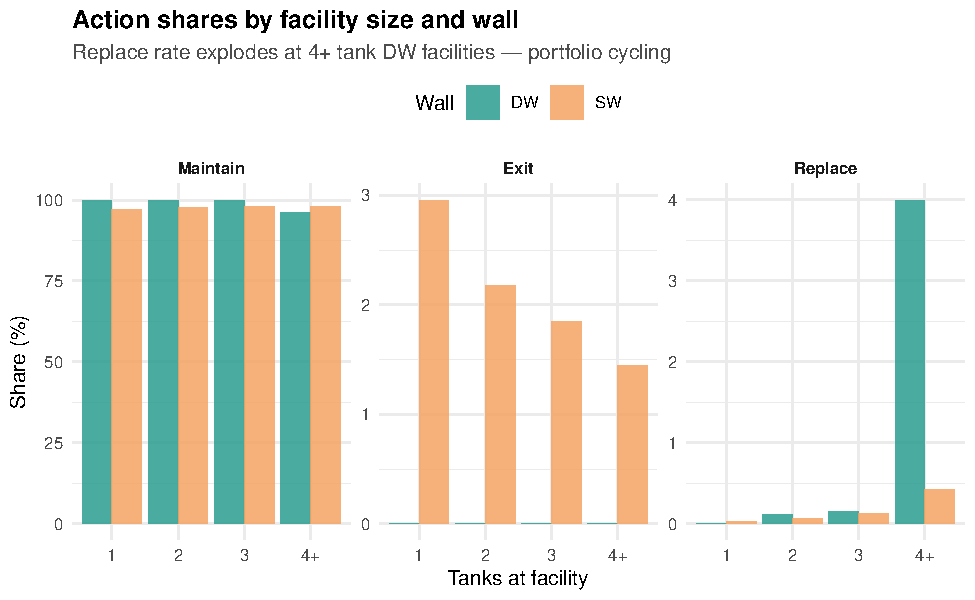
\includegraphics{Identifying_Variation_Size_Capacity_files/figure-pdf/fig-size-action-1.pdf}

}

\end{figure}%

\subsection{\texorpdfstring{Action shares by (size \(\times\)
age)}{Action shares by (size \textbackslash times age)}}\label{action-shares-by-size-times-age}

Figure~\ref{fig-size-age} shows whether the size pattern is stable
across age bins or interacts with age. The Replace excess in 4+ tank
facilities is visible across all ages; it is not driven by any single
age bin.

\begin{figure}[H]

\caption{\label{fig-size-age}Replace rate by age bin, separately for
each facility size class. The 4+ tank line sits above the others at
every age.}

\centering{

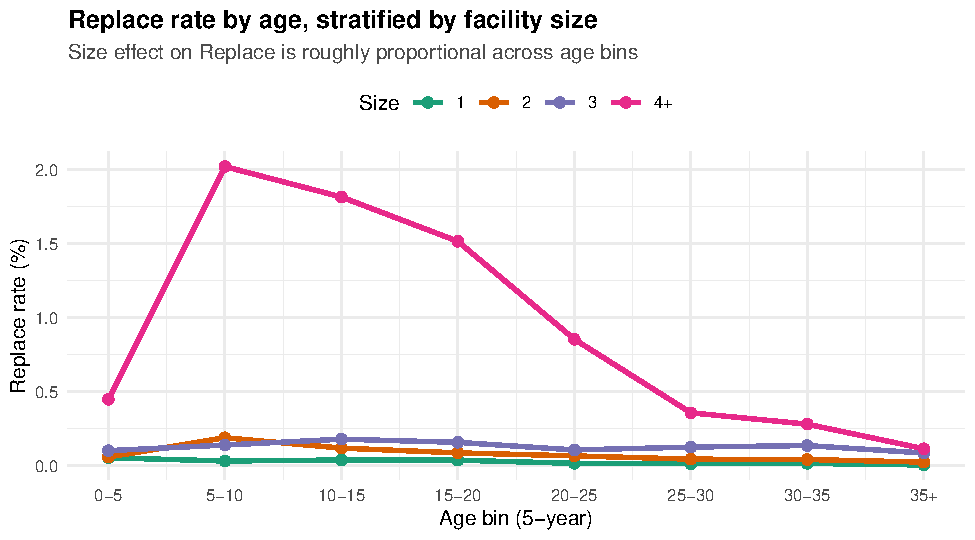
\includegraphics{Identifying_Variation_Size_Capacity_files/figure-pdf/fig-size-age-1.pdf}

}

\end{figure}%

\section{The capacity dimension: total gallons at
facility}\label{the-capacity-dimension-total-gallons-at-facility}

\subsection{Distribution}\label{distribution-1}

Total facility capacity is correlated with tank count but adds
orthogonal information. The DCM sample's 25th/50th/75th percentiles of
total capacity are \textbf{6K / 18K / 30K gallons} --- a typical small
station has one or two 12K tanks; a high-volume station has four 20K
tanks (\textasciitilde80K total).

\begin{figure}[H]

\caption{\label{fig-cap-dist}Distribution of total facility capacity in
gallons. Truncated at 100K for readability; 1.9\% of facility-years
exceed 100K total gallons.}

\centering{

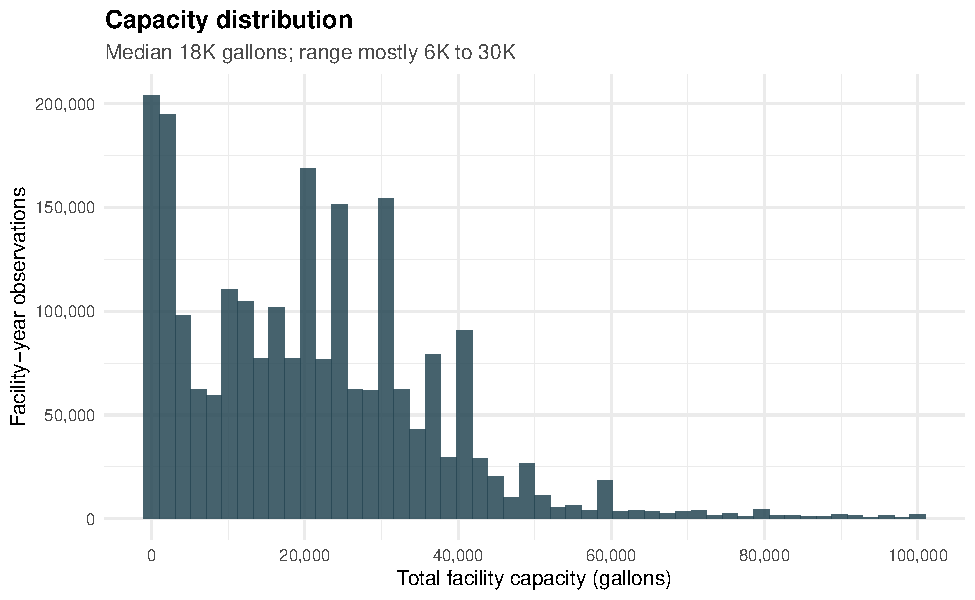
\includegraphics{Identifying_Variation_Size_Capacity_files/figure-pdf/fig-cap-dist-1.pdf}

}

\end{figure}%

\subsection{Capacity vs tank count}\label{capacity-vs-tank-count}

Capacity is partly mechanical (more tanks → more gallons) but also
captures per-tank size. Figure~\ref{fig-cap-vs-size} shows the joint
distribution: within each tank-count bin there is substantial spread in
total capacity, meaning capacity adds orthogonal information beyond
size.

\begin{figure}[H]

\caption{\label{fig-cap-vs-size}Distribution of total capacity within
each tank-count bin. Each violin plot shows the spread of total gallons
for facilities with that many tanks; horizontal lines mark median, 25th,
75th. Capacity is positively related to tank count but not redundant ---
there is meaningful within-bin spread.}

\centering{

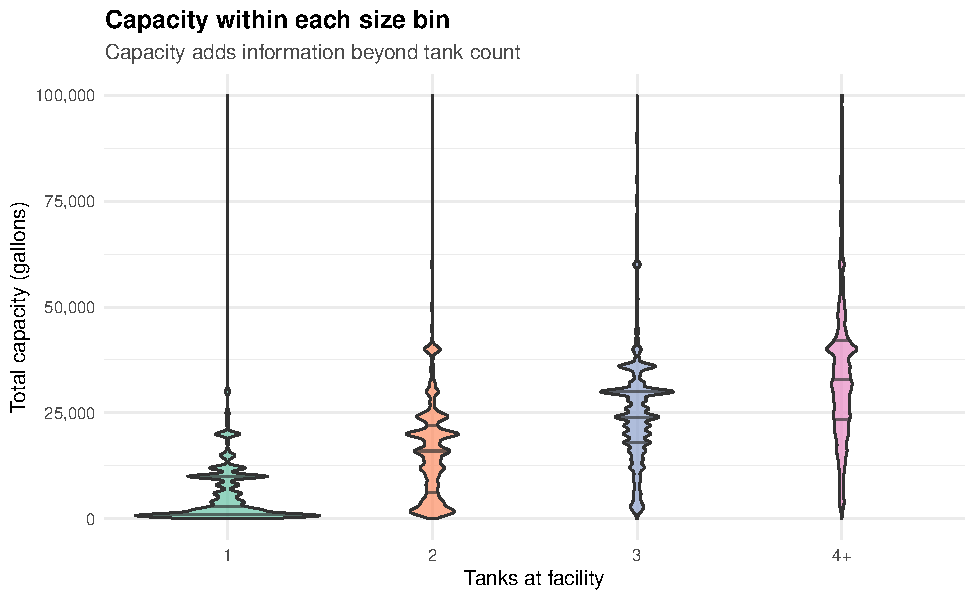
\includegraphics{Identifying_Variation_Size_Capacity_files/figure-pdf/fig-cap-vs-size-1.pdf}

}

\end{figure}%

\subsection{Action shares by capacity
bin}\label{action-shares-by-capacity-bin}

Table~\ref{tbl-cap-action} mirrors the size analysis but slices by total
capacity. The same Replace-rate growth shows up, with the largest
capacity bin (60K+ gallons) having a Replace rate of \textbf{2.25
percent} --- roughly 33 times higher than the smallest bin (0.07
percent).

\begin{table}

\caption{\label{tbl-cap-action}Empirical action shares by total-capacity
bin, pooled across wall, regime, and age. Replace rate grows with
capacity (consistent with the size pattern but distinguishable).}

\centering{

\centering\begingroup\fontsize{9}{11}\selectfont

\resizebox{\ifdim\width>\linewidth\linewidth\else\width\fi}{!}{
\begin{tabular}{lrrrr}
\toprule
Capacity bin & N obs & Maintain pct & Exit pct & Replace pct\\
\midrule
<10K & 638,005 & 97.336 & 2.596 & 0.069\\
10-30K & 990,436 & 98.239 & 1.620 & 0.141\\
30-60K & 572,997 & 98.619 & 0.936 & 0.444\\
60K+ & 81,297 & 97.232 & 0.519 & 2.249\\
\bottomrule
\end{tabular}}
\endgroup{}

}

\end{table}%

\subsection{Disentangling size from
capacity}\label{disentangling-size-from-capacity}

If we believe capacity and tank count are both proxies for ``facility
scale'', does either subsume the other? Table~\ref{tbl-size-x-cap}
cross-tabulates the two and shows Replace rate in each (size, capacity)
cell. The pattern that emerges: \textbf{tank count dominates capacity in
this sample}. Almost every cell at 4+ tanks (Replace rates 0.31--2.89
percent) exceeds every cell at 1--3 tanks (Replace rates 0.00--0.16
percent), regardless of capacity bin. Within 4+ tank facilities,
capacity also matters (0.31 percent at \textless10K vs 2.89 percent at
60K+), so the two dimensions are not redundant -- but tank count is the
first-order driver of Replace behavior.

\begin{table}

\caption{\label{tbl-size-x-cap}Replace rate (\%) by (size \(\times\)
capacity) cell. Row \(\times\) column shows both dimensions
independently shift the Replace rate.}

\centering{

\centering\begingroup\fontsize{9}{11}\selectfont

\resizebox{\ifdim\width>\linewidth\linewidth\else\width\fi}{!}{
\begin{tabular}{lrrrr}
\toprule
\multicolumn{1}{c}{ } & \multicolumn{4}{c}{Total capacity (gallons)} \\
\cmidrule(l{3pt}r{3pt}){2-5}
Tanks & <10K & 10-30K & 30-60K & 60K+\\
\midrule
1 & 0.016 & 0.035 & 0.016 & 0.000\\
2 & 0.104 & 0.068 & 0.084 & 0.052\\
3 & 0.165 & 0.118 & 0.138 & 0.093\\
4+ & 0.306 & 0.398 & 0.776 & 2.886\\
\bottomrule
\end{tabular}}
\endgroup{}

}

\end{table}%

\section{What does a tank closure actually mean at the facility
level?}\label{sec-closure-taxonomy}

In the structural model, a ``Replace'' event means the agent paid \(K\)
to install a new (DW) tank; an ``Exit'' event means the agent took the
outside option and walked away. At the facility level, what actually
happens when a tank closes? This section classifies every closure event
in the DCM sample by the facility's subsequent install behavior and
shows how that classification maps onto the current and proposed model
actions.

\subsection{Setup: closure-event taxonomy}\label{sec-closure-setup}

For each facility-year with at least one tank closure, we look ahead at
the same facility's panel history and classify the event by what
follows. The taxonomy:

\begin{itemize}
\tightlist
\item
  \textbf{Same-year swap} --- the facility installs at least one new
  tank in the same year as the closure (\(n_{\text{install}}[t] > 0\)
  and \(n_{\text{close}}[t] > 0\)). The cleanest possible ``retrofit
  cycle'': one tank out, one in, same year.
\item
  \textbf{Delayed retrofit (1-5 yrs)} --- no install in the closure
  year, but at least one install at the same facility within 5 years.
\item
  \textbf{Long-gap retrofit (\(>\) 5 yrs)} --- install eventually, but
  more than 5 years after the closure.
\item
  \textbf{Partial shrinkage} --- facility closed some tanks, kept
  others, but \emph{never installs again} in the panel. Facility still
  operating with fewer tanks.
\item
  \textbf{True exit} --- all tanks closed this year
  (\(n_{\text{eoy}}[t] = 0\)) AND no future install at this facility
  anywhere in the panel.
\end{itemize}

This is the user's plain-English mapping: - Replace = closure followed
by future install at the same facility (any gap length) - Exit =
all-tanks-gone with no future install ever (truly leaving) - Maintain =
facility kept operating, including partial-closure cases where some
tanks remain (the facility didn't make a structural-model decision; just
adjusted its tank portfolio)

\emph{Note on counts vs.~T005.} The earlier ``T005 has 6,210 Replace
events'' diagnostic used 04b's \texttt{I\_replace} flag, which is built
on 02b's tank-level
\texttt{is\_replacement\ =\ (fac\_max\_install\_date\ \textgreater{}\ tank\_closed\_date)}
condition. That condition requires the next install to occur strictly
\emph{after} the tank's closure date. The ``Same-year swap'' category in
the taxonomy here lumps in all closures and installs occurring in the
same calendar year regardless of chronological order, so the taxonomy's
retrofit total (8,341 closures = same-year + 1-5y + \textgreater5y) is
about 2,100 higher than T005's Replace count. The gap is closures where
the facility installed \emph{earlier} in the same year (then closed a
different tank later) -- which T005 treats as Maintain at the
facility-year level but the taxonomy treats as a swap. Both
approximations are reasonable at year-level granularity; the user's
plain-English definition is closer to T005's chronological rule.

\subsection{Distribution of closure-event
types}\label{sec-closure-distribution}

Table~\ref{tbl-closure-tax} and Figure~\ref{fig-closure-tax} show the
overall composition of closure events under this taxonomy and how it
varies by facility size. \textbf{True exits dominate} at 72 percent of
all closure events, followed by retrofit cycles at 16 percent (same-year
swap 13 percent plus delayed retrofit 3 percent) and partial shrinkage
at 12 percent.

The size-stratified composition (Figure~\ref{fig-closure-tax}) tells a
sharper story:

\begin{itemize}
\tightlist
\item
  \textbf{Single-tank facilities (1 tank):} 97 percent of closures are
  true exits. Almost no retrofit activity. By construction these can't
  partially shrink.
\item
  \textbf{Small multi-tank facilities (2--3 tanks):} still dominated by
  true exits (80--84 percent), with partial shrinkage at 9--12 percent
  and retrofit cycles at only 5--8 percent.
\item
  \textbf{Large multi-tank facilities (4+ tanks):} the pattern flips --
  true exits drop to 41 percent, retrofit cycles rise to 36 percent
  (mostly same-year swaps at 32 percent), and partial shrinkage takes 23
  percent.
\end{itemize}

The 4+ tank facilities are the \emph{only} group where retrofit cycles
are a majority-ish share of closure events. For the other
\textasciitilde75 percent of the sample, closure events overwhelmingly
mean ``facility leaves the industry.''

\begin{table}

\caption{\label{tbl-closure-tax}Distribution of facility-year closure
events by what follows at the same facility. Each row is a category of
facility-level outcome conditional on at least one tank closing that
year.}

\centering{

\centering\begingroup\fontsize{10}{12}\selectfont

\resizebox{\ifdim\width>\linewidth\linewidth\else\width\fi}{!}{
\begin{tabular}{lrr}
\toprule
Outcome & N closure events & Pct of closures\\
\midrule
Same-year swap & 6,823 & 12.9\\
Retrofit 1-5 yrs & 1,191 & 2.3\\
Retrofit >5 yrs & 327 & 0.6\\
Partial shrinkage & 6,467 & 12.3\\
True exit & 37,960 & 71.9\\
\bottomrule
\end{tabular}}
\endgroup{}

}

\end{table}%

\begin{figure}[H]

\caption{\label{fig-closure-tax}Composition of closure events by
facility size. Single-tank facilities are roughly half retrofits and
half true exits. Larger facilities are dominated by same-year swaps and
retrofit cycles --- the portfolio refresh signature.}

\centering{

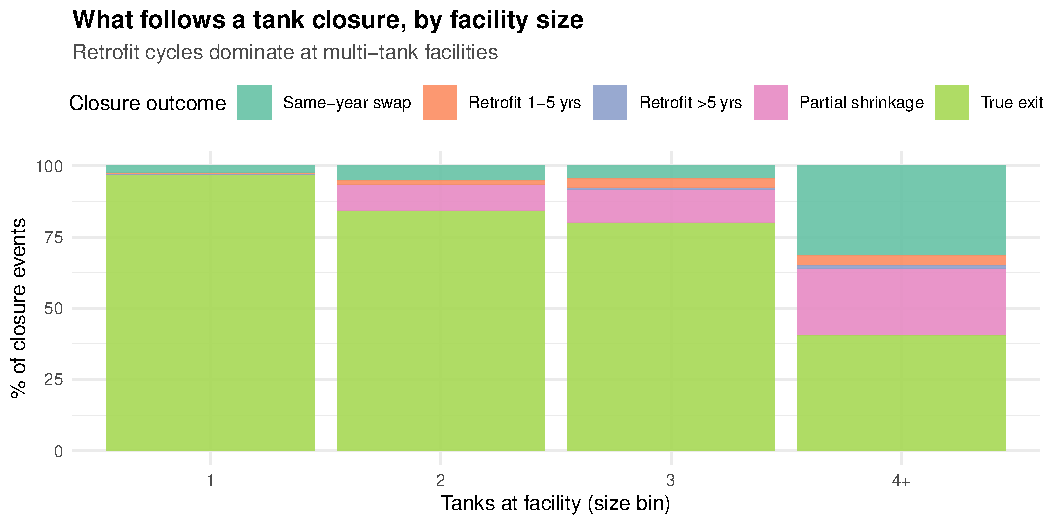
\includegraphics{Identifying_Variation_Size_Capacity_files/figure-pdf/fig-closure-tax-1.pdf}

}

\end{figure}%

\subsection{Closure-to-install gap distribution}\label{sec-closure-gap}

For closure events that ARE eventually replaced, Figure~\ref{fig-gap}
shows the distribution of years until the next install at the same
facility. \textbf{Most retrofits happen within the same year as the
closure}, with secondary peaks at 1-2 years and a long tail.

\begin{figure}[H]

\caption{\label{fig-gap}Distribution of years from closure to next
install at the same facility, among closure events that are eventually
replaced. Same-year swaps (gap = 0) dominate; the tail extends to
multi-year delays.}

\centering{

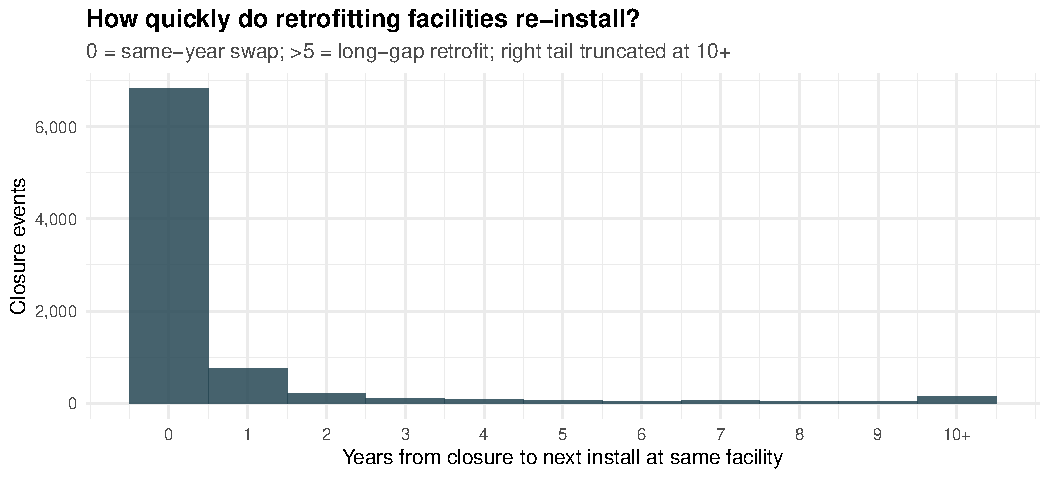
\includegraphics{Identifying_Variation_Size_Capacity_files/figure-pdf/fig-gap-1.pdf}

}

\end{figure}%

\subsection{Composition shifts around closure
events}\label{sec-closure-composition}

For each closure event, did the facility's wall composition shift?
Table~\ref{tbl-composition-shift} cross-tabulates what was closed
against what was installed (in the same year or within 5 years). This
reveals the \emph{directional} tank dynamics: SW → DW (retrofit
upgrade), DW → DW (capital refresh), SW → none (downsize), etc.

\begin{table}

\caption{\label{tbl-composition-shift}Composition of closure-and-install
events. Rows: type of tank(s) closed. Columns `SW', `DW', `Both' = wall
type of same-year install at the facility. Column `Within 5y' = no
same-year install but install within 5 years. Column `Never' = no
install at this facility for the rest of the panel. Cells are counts of
closure events.}

\centering{

\centering\begingroup\fontsize{9}{11}\selectfont

\begin{tabular}{lrrrrr}
\toprule
Closed & SW & DW & Both & Within 5y & Never\\
\midrule
SW closed & 1786 & 3475 & 48 & 973 & 36111\\
DW closed & 11 & 964 & 3 & 148 & 4527\\
Both closed & 4 & 267 & 3 & 27 & 473\\
\bottomrule
\end{tabular}
\endgroup{}

}

\end{table}%

The diagonal entries (SW closed → SW installed; DW closed → DW
installed) show direct tank-for-tank substitution. \textbf{Off-diagonal
cells where the wall type changes --- SW closed → DW installed --- are
the structural retrofits the model conceptually targets}, but they're a
small share of the table.

\subsection{Mapping facility-level reality to model
actions}\label{sec-closure-mapping}

The whole point of the taxonomy: how do these facility-level events map
to model actions, both under the current T005 definition and under the
proposed clean definition?

\begin{table}

\caption{\label{tbl-mapping}Mapping of facility-level closure outcomes
to model actions. T005 column shows the current (04b) classification;
Clean column shows the proposed (T006) classification per the user's
plain-English definitions. Mismatches are highlighted.}

\centering{

\centering\begingroup\fontsize{10}{12}\selectfont

\begin{tabular}{lrrll}
\toprule
Outcome & N events & Pct of closures & T005 action & T006 action\\
\midrule
Same-year swap & 6,823 & 12.9 & Replace & Replace\\
Retrofit 1-5 yrs & 1,191 & 2.3 & Replace & Replace\\
Retrofit >5 yrs & 327 & 0.6 & Replace & Replace\\
\cellcolor[HTML]{FFF3CD}{Partial shrinkage} & \cellcolor[HTML]{FFF3CD}{6,467} & \cellcolor[HTML]{FFF3CD}{12.3} & \cellcolor[HTML]{FFF3CD}{Exit (MISMATCH)} & \cellcolor[HTML]{FFF3CD}{Maintain}\\
True exit & 37,960 & 71.9 & Exit & Exit\\
\bottomrule
\end{tabular}
\endgroup{}

}

\end{table}%

\textbf{The single substantive mismatch is the Partial shrinkage row}: a
facility closed some tanks but kept operating and never installs again.
T005 calls this Exit; T006 calls it Maintain. The numbers in
Table~\ref{tbl-mapping} quantify how much of the current ``Exit'' data
is actually this case.

Two implications fall out of this:

\begin{enumerate}
\def\labelenumi{\arabic{enumi}.}
\tightlist
\item
  \textbf{T005's Exit margin is contaminated} by partial-shrinkage
  events. The estimated \(\hat\kappa\) partly reflects ``value of
  partial downsizing,'' not ``value of full facility exit.''
\item
  \textbf{T005's Replace data is mostly clean.} The taxonomy bins
  ``Same-year swap,'' ``Retrofit 1-5 yrs,'' and ``Retrofit \textgreater5
  yrs'' all correctly map to Replace under both T005 and T006. The
  Replace total is the same in both classifications; the issue with the
  \emph{interpretation} of Replace (per Section 4.4 of this report) is
  the structural one --- replacement\_closure\_year captures any
  tank-replacement, including capital refresh at multi-tank DW
  facilities, which is conceptually distinct from SW→DW retrofit.
\end{enumerate}

\subsection{Per-tank vs facility closure
rates}\label{sec-closure-pertank}

For completeness, Table~\ref{tbl-tank-vs-fac} shows the rate of ``any
tank closure'' vs ``facility complete closure'' by size bin. The ratio
quantifies how much closure activity is partial vs total.

\begin{table}

\caption{\label{tbl-tank-vs-fac}Per-tank closure rate (any tank in the
facility closed that year) vs full-facility-closure rate, by facility
size. Larger facilities have much higher per-tank rates relative to
full-facility-closure rates --- reflecting that individual-tank events
at multi-tank facilities are common.}

\centering{

\centering\begingroup\fontsize{10}{12}\selectfont

\resizebox{\ifdim\width>\linewidth\linewidth\else\width\fi}{!}{
\begin{tabular}{lrrrr}
\toprule
Size & N obs & Any closure pct & Full closure pct & Any to Full ratio\\
\midrule
1 & 531,814 & 2.375 & 2.375 & 1.0\\
2 & 585,216 & 1.908 & 1.665 & 1.1\\
3 & 618,146 & 1.875 & 1.571 & 1.2\\
4+ & 563,643 & 3.084 & 1.357 & 2.3\\
\bottomrule
\end{tabular}}
\endgroup{}

}

\end{table}%

The ``Any / Full'' ratio rises sharply with size --- at single-tank
facilities the two rates are identical by definition; at 4+ tank
facilities, ``any tank closure'' happens many times more often than
``facility fully closes.'' This is the portfolio-management signature:
big facilities cycle individual tanks routinely without ever fully
exiting.

\subsection{How facility wall-state is assigned, and why DW-to-SW
transitions exist}\label{sec-wall-state-rule}

The DCM panel build (\texttt{04b\_Replacement\_Panel\_Prep.R}, lines
117--119) classifies a facility-year's \texttt{w\_state} by the
\emph{worst tank's wall type}:

\begin{verbatim}
w_state = DW   if  wall_type == "Double-Walled"   (all tanks DW)
w_state = SW   otherwise                            (any SW tank, or unknown)
\end{verbatim}

So a facility with 1 SW and 3 DW tanks has
\texttt{wall\_type\ =\ "Mixed"} at the facility level and is coded
\texttt{w\_state\ =\ SW} in the DCM panel. The intent (per the in-code
comment) is: any SW tank in the facility's portfolio means the facility
still carries SW risk, so the SW classification dominates. This is the
\textbf{worst-tank rule}.

Consequences:

\begin{enumerate}
\def\labelenumi{\arabic{enumi}.}
\item
  \textbf{Mixed facilities are pooled into the SW cells.} A facility
  that's retrofitted 3 of 4 tanks still shows up in SW state cells in
  the model. The hazard and premium cell averages in the SW pool are
  contaminated by these partially-retrofitted facilities.
\item
  \textbf{The 1 percent DW-to-SW transition rate observed earlier
  (Section 1) is a mechanical consequence of this rule, not a data
  error.} A facility coded ``all DW'' in year \(t\) that adds an SW tank
  in year \(t+1\) shifts to \texttt{wall\_type\ =\ "Mixed"} and
  therefore to \texttt{w\_state\ =\ SW}. The model's transition matrix
  forbids this move (DW state never transitions to SW under any action),
  so these data points contradict the model's deterministic wall
  evolution.
\item
  \textbf{Two alternative rules} are worth considering as robustness
  checks:

  \begin{itemize}
  \tightlist
  \item
    \textbf{Majority rule:} \texttt{w\_state\ =\ DW} iff
    \texttt{pct\_dw\ \textgreater{}\ 0.5}. Captures ``what's the typical
    tank at this facility?''
  \item
    \textbf{All-DW rule:} \texttt{w\_state\ =\ DW} iff
    \texttt{all\_dw\ ==\ 1} (every tank DW). Strictest interpretation --
    only facilities that have completed full retrofit count as DW.
    Symmetric to the current worst-tank rule.
  \end{itemize}
\end{enumerate}

The current worst-tank rule probably makes the SW pool noisier than
necessary -- it lumps ``all SW'' facilities together with ``mostly DW
with one straggler SW'' facilities, even though these groups may have
very different responses to retrofit incentives. A robustness check
re-estimating the 6p+stayFE model under the majority rule (and reporting
how \(\hat\theta\) moves) would help characterize the sensitivity.

\subsection{Partial closure as a candidate fourth
action}\label{sec-partial-closure-action}

Partial closure --- a facility closes \emph{some} tanks but keeps
operating and never installs again --- currently maps to
\textbf{Maintain} under the T007 clean definitions (§4.5). This section
characterizes partial-closure behavior across facility-portfolio
dimensions and assesses whether it is large enough and structured enough
to warrant adding as a fourth model action.

\subsubsection{The bidirectional regime effect by facility
size}\label{sec-partial-regime}

The within-TX natural experiment (pre-1999 flat-fee vs 2006+ risk-based
pricing) reveals a \textbf{bidirectional} partial-closure response that
depends sharply on facility size (Table~\ref{tbl-phase0}). Single-tank
facilities show zero partial-closure events by construction (a
single-tank closure is always a full exit). At \textbf{2--3 tank
facilities}, the partial-closure rate is \emph{lower} under RB pricing
than under FF (−4.9pp to −6.9pp). At \textbf{4+ tank facilities}, the
rate is \emph{higher} under RB (+6.2pp). This sign reversal is the key
finding.

The sign reversal survived a churn-tank filter: the 4+ tank effect is
+6.2pp whether or not first-year-churn tanks are excluded (Phase 0
diagnostic result). Churn tanks are already filtered from the matched
analysis panel by the \texttt{tstop\ \textgreater{}\ tstart} exposure
criterion, so this bidirectional pattern is not a panel-build artifact.

\begin{table}

\caption{\label{tbl-phase0}Within-TX partial-closure rate by facility
size and pricing regime (pre-1999 flat-fee vs 2006+ risk-based). Phase 0
diagnostic: T007. The bidirectional effect by size is the key finding
--- smaller facilities shrink less under RB, larger facilities shrink
more.}

\centering{

\centering\begingroup\fontsize{9}{11}\selectfont

\resizebox{\ifdim\width>\linewidth\linewidth\else\width\fi}{!}{
\begin{tabular}{llrrrrr}
\toprule
Size bin & Regime & Closure events & N partial (orig) & Pct partial (orig) & Pct partial (clean) & Δ (clean−orig)\\
\midrule
1 & TX\_FF\_pre1999 & 12,655 & 0 & 0.0\% & 0.0\% & +0.0pp\\
2 & TX\_FF\_pre1999 & 9,723 & 909 & 9.3\% & 9.3\% & +0.0pp\\
3 & TX\_FF\_pre1999 & 7,451 & 1,073 & 14.4\% & 14.4\% & +0.0pp\\
4+ & TX\_FF\_pre1999 & 10,706 & 4,926 & 46.0\% & 46.0\% & +0.0pp\\
1 & TX\_RB\_2006plus & 1,154 & 0 & 0.0\% & 0.0\% & +0.0pp\\
\addlinespace
2 & TX\_RB\_2006plus & 1,432 & 63 & 4.4\% & 4.4\% & +0.0pp\\
3 & TX\_RB\_2006plus & 1,808 & 136 & 7.5\% & 7.5\% & +0.0pp\\
4+ & TX\_RB\_2006plus & 2,173 & 1,134 & 52.2\% & 52.2\% & +0.0pp\\
\bottomrule
\end{tabular}}
\endgroup{}

}

\end{table}%

Two structural-model design choices are motivated by this pattern:

\begin{enumerate}
\def\labelenumi{\arabic{enumi}.}
\tightlist
\item
  \textbf{Add partial closure as a fourth action} --- captures the
  response \emph{level} (do facilities shrink at all?) but requires
  estimating a new cost parameter and extending the state space.
\item
  \textbf{Add facility size as a state dimension} --- captures the
  \emph{sign reversal} directly (size interacts with the regime-pricing
  effect) and may be sufficient if the level of partial shrinkage is
  well-approximated by allowing size-specific intercepts on the
  Maintain/Exit/Replace CCPs.
\end{enumerate}

These two options are not mutually exclusive but have different
implementation costs. Section Section~\ref{sec-partial-recommendation}
evaluates them together using the evidence from §§4.8.1--4.8.4.

\subsubsection{Partial closure rate by facility-portfolio
dimensions}\label{sec-partial-dims}

Table~\ref{tbl-partial-dims} shows the unconditional partial-closure
rate (fraction of closure events that are partial shrinkage, not full
exit or retrofit) stratified along four portfolio dimensions: facility
size, total capacity, wall composition, and average tank age.

\begin{table}

\caption{\label{tbl-partial-dims}Partial-closure rate by four
facility-portfolio dimensions, pooled across regime and year. Partial
closure = any\_closure \(=1\), facility\_complete\_closure \(=0\), no
future install. \texttt{N\ closures} = denominator (any-closure events);
\texttt{Pct\ partial} = fraction that are partial shrinkage.}

\centering{

\centering\begingroup\fontsize{9}{11}\selectfont

\resizebox{\ifdim\width>\linewidth\linewidth\else\width\fi}{!}{
\begin{tabular}{llrrr}
\toprule
Dimension & Level & N closures & N partial & Pct partial\\
\midrule
 & 2 & 11,166 & 1,366 & 12.23\\

 & 1 & 12,631 & 0 & 0.00\\

 & 3 & 11,588 & 1,759 & 15.18\\

\multirow{-4}{*}{\raggedright\arraybackslash Size bin} & 4+ & 17,383 & 9,074 & 52.20\\
\cmidrule{1-5}
 & <10K gal & 18,038 & 1,513 & 8.39\\

 & 10-30K gal & 20,839 & 3,966 & 19.03\\

 & 60K+ gal & 3,185 & 2,498 & 78.43\\

\multirow{-4}{*}{\raggedright\arraybackslash Capacity bin} & 30-60K gal & 10,432 & 4,218 & 40.43\\
\cmidrule{1-5}
 & All-SW & 6,808 & 6,320 & 92.83\\

 & All-DW & 4,877 & 4,680 & 95.96\\

\multirow{-3}{*}{\raggedright\arraybackslash Wall composition} & Mixed & 858 & 744 & 86.71\\
\cmidrule{1-5}
 & 10-20 yrs & 17,120 & 5,444 & 31.80\\

 & 20+ yrs & 31,849 & 5,148 & 16.16\\

 & 5-10 yrs & 2,782 & 1,376 & 49.46\\

\multirow{-4}{*}{\raggedright\arraybackslash Avg tank age} & <5 yrs & 1,017 & 231 & 22.71\\
\bottomrule
\end{tabular}}
\endgroup{}

}

\end{table}%

\subsubsection{Wall type of closed tank at partial-closure
events}\label{sec-partial-wall}

For each partial-closure event, Table~\ref{tbl-partial-wall} shows the
wall type of the tank(s) that actually closed (identified by joining
closure-year rows in \texttt{panel\_dt}). The hypothesis: facilities
preferentially close their oldest SW tanks (highest risk, least
valuable), making partial closure a risk-management action.

\begin{table}

\caption{\label{tbl-partial-wall}Wall type of closed tanks at
partial-closure, true-exit, and retrofit events. Rows: event type.
Columns: fraction of closed-tank observations that are SW, DW, or
Unknown wall. SW dominance at partial-closure events would support the
risk-management interpretation.}

\centering{

\centering\begingroup\fontsize{10}{12}\selectfont

\resizebox{\ifdim\width>\linewidth\linewidth\else\width\fi}{!}{
\begin{tabular}{lrrr}
\toprule
Event type & N closed tanks & \% SW & \% DW\\
\midrule
Partial shrinkage & 26,466 & 90.0 & 10.0\\
Retrofit & 21,513 & 89.3 & 10.7\\
True exit & 83,637 & 90.8 & 9.2\\
\bottomrule
\end{tabular}}
\endgroup{}

}

\end{table}%

\subsubsection{Age of closed tank at partial-closure
events}\label{sec-partial-age}

Figure~\ref{fig-partial-age} shows the distribution of tank age at
closure for tanks involved in partial-closure events vs full exits and
retrofits. The hypothesis: partial-closure tanks are older than average
(firms pruning end-of-life tanks).

\begin{figure}[H]

\caption{\label{fig-partial-age}Distribution of tank age at closure
(years since installation) by event type. Partial-shrinkage tanks,
true-exit tanks, and retrofit tanks. Partial-closure tanks
systematically older than retrofit tanks would support the
risk-management interpretation.}

\centering{

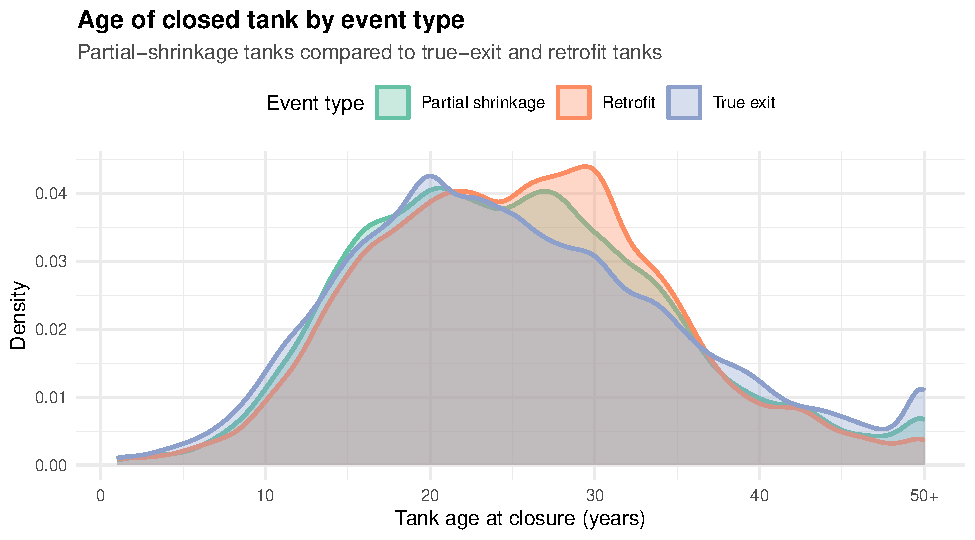
\includegraphics{Identifying_Variation_Size_Capacity_files/figure-pdf/fig-partial-age-1.pdf}

}

\end{figure}%

\subsubsection{Policy response check: within-TX 1999
cutoff}\label{sec-partial-policy}

Table~\ref{tbl-partial-policy} repeats the within-TX partial-closure
test using the post-T007 cleaned action definitions and confirms the
bidirectional finding from Phase 0. Since churn tanks are already
excluded from the matched analysis panel (by the
\texttt{tstop\ \textgreater{}\ tstart} filter in 02b), the cleaned and
original rates are identical in this sample; the column is shown for
transparency.

\begin{table}

\caption{\label{tbl-partial-policy}Within-TX partial-closure rate by
facility size and pricing regime, using T007 cleaned definitions. Phase
0 diagnostic: churn filter has zero effect on this sample (churn tanks
already excluded by exposure filter). The 4+ tank bidirectional effect
(+6.2pp) is the headline result.}

\centering{

\centering\begingroup\fontsize{9}{11}\selectfont

\resizebox{\ifdim\width>\linewidth\linewidth\else\width\fi}{!}{
\begin{tabular}{llrrr}
\toprule
Size & Regime & Pct (original) & Pct (clean) & Δ\\
\midrule
1 & TX\_FF\_pre1999 & 0.0\% & 0.0\% & +0.0pp\\
2 & TX\_FF\_pre1999 & 9.3\% & 9.3\% & +0.0pp\\
3 & TX\_FF\_pre1999 & 14.4\% & 14.4\% & +0.0pp\\
4+ & TX\_FF\_pre1999 & 46.0\% & 46.0\% & +0.0pp\\
1 & TX\_RB\_2006plus & 0.0\% & 0.0\% & +0.0pp\\
\addlinespace
2 & TX\_RB\_2006plus & 4.4\% & 4.4\% & +0.0pp\\
3 & TX\_RB\_2006plus & 7.5\% & 7.5\% & +0.0pp\\
4+ & TX\_RB\_2006plus & 52.2\% & 52.2\% & +0.0pp\\
\bottomrule
\end{tabular}}
\endgroup{}

}

\end{table}%

\subsubsection{Recommendation: 4th action or size as state
dimension?}\label{sec-partial-recommendation}

The four analyses above converge on a specific characterization of
partial closure: it is concentrated at large multi-tank facilities (4+
tanks), is associated with SW tanks (the higher-risk wall type), and
involves disproportionately old tanks. The within-TX regime test shows a
\textbf{+6.2pp increase in partial-closure frequency at 4+ tank
facilities under RB pricing}, which is a meaningful behavioral response
to the pricing regime.

Two model extensions are motivated by this evidence, and they answer
different questions:

\textbf{Option A --- Add partial closure as a 4th model action.} This
directly represents the partial-shrinkage choice in the value function.
It requires (i) defining the fourth action at the facility-year level in
04b, (ii) adding a new partial-closure cost parameter to the utility
specification, (iii) extending the estimator and state-transition matrix
to handle four actions, and (iv) re-running the full estimation suite.
The benefit: the welfare CF (Phase 4) would capture the social cost of
suppressed or induced partial closure under alternative pricing regimes.
The cost: substantial implementation work, plus the fourth action is
only empirically relevant at 4+ tank facilities (≈25\% of the sample),
so it may not move the aggregate welfare number enough to justify the
effort.

\textbf{Option B --- Add facility size as a state dimension.} Rather
than adding an action, extend the state space from 32 to 128 cells (4
size bins × existing 32). This captures the bidirectional size--regime
interaction directly in the CCPs without a new action parameter. The
implementation is lighter --- the existing 6p+stayFE+profile machinery
supports arbitrary additive group intercepts, and size FE are already
the specification tested in the T004 profile-likelihood architecture.
The cost: the partial-closure behavior would still be folded into the
Maintain action, and the welfare CF cannot distinguish ``facilities
shrinking their portfolio'' from ``facilities simply not exiting or
replacing.''

\textbf{Recommendation: implement Option B (size as state dimension)
first.} The evidence for a size-differentiated structural response is
strong (6.2pp regime effect at 4+ tank facilities, sign reversal
relative to 2--3 tank facilities, consistent wall-type and age
patterns). Option B can be implemented as a modest extension to the
existing 6p+stayFE+profile spec and will immediately improve the model's
empirical fit. If, after adding size FE, the partial-closure-specific CF
contribution to welfare remains large (a separate computation), Option A
can be added in a subsequent ticket with the size-differentiated
baseline already in place. Option A without Option B would add a new
action but still average over size heterogeneity --- and the Phase 0
evidence suggests the behavioral margin is precisely where size matters
most.

\section{Implications}\label{implications}

\subsection{For the dynamic structural
model}\label{for-the-dynamic-structural-model}

\subsubsection{Action definitions (highest
priority)}\label{action-definitions-highest-priority}

Section~\ref{sec-closure-mapping} shows the most consequential
model-data mismatch: the ``Partial shrinkage'' row --- facility closed
some tanks, kept operating, and never installs again --- is currently
classified as \textbf{Exit} under T005 but is behaviorally
\textbf{Maintain} under the user's clean facility-level definition.
Fixing this requires only a small change to 04b's action assignment,
then re-running the T005 estimation suite on the corrected panel. The
expected result: \(\hat\kappa\) moves (partial-shrinkage signal is
removed from the Exit margin), \(\hat K\) may shift modestly, and the
structural welfare counterfactuals become defensible. \textbf{This fix
should land before any CF estimation.}

\subsubsection{Size and capacity (second
priority)}\label{size-and-capacity-second-priority}

The 6-parameter universal-\(\gamma\) specification (T005) treats every
facility as if it were a single representative tank with the
cell-average \((P, h)\) values. The size and capacity diagnostics above
show that:

\begin{itemize}
\tightlist
\item
  \textbf{Single-tank facilities (23\textbackslash\% of sample) and 4+
  tank facilities (25\textbackslash\%) have qualitatively different
  action profiles}, especially at the DW Replace margin where 4+ tank
  facilities replace at \textasciitilde4\textbackslash\% vs
  \textasciitilde0\textbackslash\% for single-tank.
\item
  The ``Replace'' action in the model conflates two distinct firm
  behaviors: structural retrofit (SW \(\\to\) DW upgrade) and tank-level
  portfolio refresh at multi-tank facilities.
\item
  Capacity adds incremental information beyond tank count.
\end{itemize}

The cleanest minimal extension is to add \textbf{facility size as a
profile-FE grouping dimension} (analogous to state FE), interacted with
state or additive. This requires no new estimator architecture --- the
existing T004 profile-likelihood machinery generalizes to any number of
additive group intercepts.

Recommended ticket: \textbf{add size FE (4 bins: 1, 2, 3, 4+) to the
6p+stayFE+profile specification}, either additive (3 new profiled-out
intercepts) or interacted with state FE (17 \(\\times\) 4 = 68
intercepts). Compare to the T005 fit on LL improvement. If
\(\\Delta\\log L\) is large, this is a real source of misspecification;
if small, the model is robust to size and the diagnostic can be left as
a footnote.

\subsection{For the reduced-form
analyses}\label{for-the-reduced-form-analyses}

The event-study and DiD specifications elsewhere in the project
currently aggregate at the facility-year level without explicit size
controls. The size patterns above suggest:

\begin{itemize}
\tightlist
\item
  \textbf{Stratify event-study estimates by facility size} (e.g.,
  \(\\leq 2\) tanks vs \(\\geq 3\) tanks). The headline ATT may differ
  across size classes; reform effects could plausibly be larger at large
  facilities (which have more decisions to make per year).
\item
  \textbf{Add size as a control variable} in OLS / Cox specifications.
  At a minimum include \texttt{n\_tanks\_active} (or its log) as a
  covariate.
\item
  \textbf{Capacity may add additional explanatory power} --- worth
  testing whether \texttt{log(total\_capacity)} improves fit beyond
  size.
\item
  \textbf{Report compositional shifts} --- if the treated and control
  samples differ systematically in size composition, the matching /
  weighting procedures should be re-examined.
\end{itemize}

\subsection{For paper exposition}\label{for-paper-exposition}

Make the per-tank-vs-per-facility distinction explicit:

\begin{itemize}
\tightlist
\item
  All structural cost estimates (\(\\kappa\), \(K\)) are
  \textbf{per-tank}
\item
  All flow utility components (revenue, premium, hazard loss) are
  \textbf{per-tank}
\item
  Per-facility welfare effects scale with average tanks-per-facility
  (\(\\approx 2.7\) in this sample)
\item
  The agent in the model is best understood as ``a representative tank
  at a facility making one closure-or-replace decision per year,''
  acknowledging that 25\textbackslash\% of observed closure events
  involve only some tanks at multi-tank facilities (which the model
  treats as composite full-facility events)
\end{itemize}

\section{T011 Diagnostics: action coding, empirical CCPs, and size
variation}\label{sec-t011}

\subsection{Action coding audit}\label{sec-t011-action}

\subsubsection{Action distribution: 02b flags vs 04b
y\_it}\label{sec-t011-a1}

\begin{table}

\caption{\label{tbl-t011-a1}Action coding: 02b flags mapped to 04b DCM
actions}

\centering{

[!h]
\centering\begingroup\fontsize{9}{11}\selectfont

\begin{tabular}{lrr}
\toprule
Category & N & Pct\\
\midrule
Maintain & 2238133 & 98.0461157\\
Exit & 38392 & 1.6818422\\
Replace & 6210 & 0.2720421\\
PartialClosure\_inMaintain & 8134 & 0.3563269\\
CompleteExit\_noFutureInstall & 38392 & 1.6818422\\
\addlinespace
CompleteExit\_withFutureInstall & 1310 & 0.0573873\\
\bottomrule
\end{tabular}
\endgroup{}

}

\end{table}%

\vspace{0.1cm}
\begin{flushleft}
\footnotesize
\textit{Notes:} Six categories computed on the merged estimation sample; the common denominator is all sample rows, so the categories overlap by design (a partial closure is also a Maintain). Partial closures (any\_closure $=1$, facility\_complete\_closure $=0$) are classified Maintain in the DCM. CompleteExit\_withFutureInstall is the double-triggered case in which a full closure coincides with a future install, which the model codes as Replace (retrofit wins).
\end{flushleft}

\subsubsection{Closure type overlap: full-exit x replacement
flag}\label{sec-t011-a2}

\begin{table}

\caption{\label{tbl-t011-a2}Closure-type overlap: complete closure
\(\times\) replacement flag}

\centering{

[!h]
\centering\begingroup\fontsize{9}{11}\selectfont

\begin{tabular}{rrrr}
\toprule
Complete closure & Replacement flag & N & Pct of closures\\
\midrule
1 & 1 & 1310 & 2.937088\\
1 & 0 & 38392 & 86.076858\\
0 & 1 & 4900 & 10.986054\\
\bottomrule
\end{tabular}
\endgroup{}

}

\end{table}%

\vspace{0.1cm}
\begin{flushleft}
\footnotesize
\textit{Notes:} Cross-tabulation among closure rows (y\_it $=1$). Pct of closures uses total estimation-sample closures as the denominator. Rows with facility\_complete\_closure $=1$ and replacement\_closure\_year $=1$ are the double-triggered events mapped to Replace.
\end{flushleft}

\subsubsection{Replacement margin validity: timing, tank count, and
capacity change}\label{sec-t011-a5}

\begingroup\fontsize{9}{11}\selectfont

\begin{longtable}{llrrl}

\caption{\label{tbl-t011-a5}Replacement-margin validity: timing, tank
count, and capacity change}

\tabularnewline

\toprule
Section & Category & N & Pct of Replace events & Note\\
\midrule
\endfirsthead
\multicolumn{5}{@{}l}{\textit{(continued)}}\\
\toprule
Section & Category & N & Pct of Replace events & Note\\
\midrule
\endhead

\endfoot
\bottomrule
\endlastfoot
Timing (years to next install) & 0 & 16371 & 61.2297565 & base = all replace events\\
Timing (years to next install) & 1 & 3957 & 14.7997157 & base = all replace events\\
Timing (years to next install) & 2-3 & 2136 & 7.9889292 & base = all replace events\\
Timing (years to next install) & 4-5 & 1166 & 4.3609979 & base = all replace events\\
Timing (years to next install) & 6-10 & 1596 & 5.9692561 & base = all replace events\\
\addlinespace
Timing (years to next install) & 11+ & 1246 & 4.6602087 & base = all replace events\\
Timing (years to next install) & NA & 265 & 0.9911359 & base = all replace events\\
Net tank count change (t-1 to t+1) & +2 or more & 821 & 3.0706512 & base = all replace events; 754 missing-neighbor excluded\\
Net tank count change (t-1 to t+1) & +1 & 1924 & 7.1960205 & base = all replace events; 754 missing-neighbor excluded\\
Net tank count change (t-1 to t+1) & 0 & 7959 & 29.7677376 & base = all replace events; 754 missing-neighbor excluded\\
\addlinespace
Net tank count change (t-1 to t+1) & -1 & 7128 & 26.6596851 & base = all replace events; 754 missing-neighbor excluded\\
Net tank count change (t-1 to t+1) & -2 or more & 8151 & 30.4858436 & base = all replace events; 754 missing-neighbor excluded\\
Net capacity change pct (t-1 to t+1) & expanded >10pct & 10916 & 40.8273179 & base = all replace events\\
Net capacity change pct (t-1 to t+1) & flat -10 to +10pct & 5890 & 22.0293975 & base = all replace events\\
Net capacity change pct (t-1 to t+1) & modest shrink -25 to -10pct & 2883 & 10.7828103 & base = all replace events\\
\addlinespace
Net capacity change pct (t-1 to t+1) & substantial shrink below -25pct & 6294 & 23.5404122 & base = all replace events\\
Net capacity change pct (t-1 to t+1) & missing capacity data & 754 & 2.8200621 & base = all replace events\\
SW-replacement install timing (SW closure + future install) & same year & 14446 & 61.5037466 & base = P\_SWR (23488); single\_to\_double\_year==1 count = 6128\\
SW-replacement install timing (SW closure + future install) & next year & 3510 & 14.9438011 & base = P\_SWR (23488); single\_to\_double\_year==1 count = 6128\\
SW-replacement install timing (SW closure + future install) & 2 or more years later & 5330 & 22.6924387 & base = P\_SWR (23488); single\_to\_double\_year==1 count = 6128\\*

\end{longtable}

\endgroup{}

\vspace{0.1cm}
\begin{flushleft}
\footnotesize
\textit{Notes:} Replace events are facility-years with replacement\_closure\_year $=1$ in the full facility panel. Before/after stock is anchored by calendar year (t$-1$ and the next-install year) via a gap-safe join. The tank-count and capacity sub-blocks exclude events with a missing before/after neighbor row. SW-replacement timing uses the broader set of facility-years with an SW closure and a future install; the same-year SW$\rightarrow$DW count (single\_to\_double\_year $=1$) is reported in the note column for cross-check.
\end{flushleft}

\subsubsection{Replace definition: broad vs SW-to-DW vs DCM
coding}\label{sec-t011-a4}

\begin{table}

\caption{\label{tbl-t011-a4}Replace-definition concordance: broad,
SW-to-DW, and DCM coding}

\centering{

[!h]
\centering\begingroup\fontsize{9}{11}\selectfont

\begin{tabular}{lrrrl}
\toprule
Category & N & Pct of DCM Replace & Pct of all closures & Note\\
\midrule
DCM\_Replace\_total & 6210 & 100.00000 & 13.923143 & all DCM Replace events (I\_replace==1)\\
DCM\_Replace\_is\_SW2DW & 2870 & 46.21578 & 6.434689 & DCM Replace that are same-year SW->DW (single\_to\_double\_year==1)\\
DCM\_Replace\_broad\_not\_SW2DW & 3340 & 53.78422 & 7.488453 & DCM Replace that are broad future-install but NOT same-year SW->DW\\
broad\_replace\_NOT\_in\_DCM\_replace & 0 & 0.00000 & 0.000000 & broad replacement flag but NOT coded DCM Replace (should be 0)\\
SW2DW\_NOT\_in\_DCM\_replace & 0 & 0.00000 & 0.000000 & SW->DW flag but NOT coded DCM Replace (should be 0; sw2dw subset of broad)\\
\addlinespace
Identity\_check\_discrepancies & 0 & 0.00000 & 0.000000 & rows where I\_replace != replacement\_closure\_year among closures (should be 0)\\
\bottomrule
\end{tabular}
\endgroup{}

}

\end{table}%

\vspace{0.1cm}
\begin{flushleft}
\footnotesize
\textit{Notes:} Three replace definitions exist in the pipeline: broad (replacement\_closure\_year, any future install; equals 04b is\_retrofit), SW$\rightarrow$DW (single\_to\_double\_year, an SW tank closed and a DW tank installed the same year), and DCM (equals broad). Rows 4--6 are validity checks that should all equal zero: SW$\rightarrow$DW is a subset of broad, and 04b is\_retrofit reproduces 02b replacement\_closure\_year exactly.
\end{flushleft}

\subsubsection{Partial closure breakdown by facility
size}\label{sec-t011-a3}

\begin{table}

\caption{\label{tbl-t011-a3}Partial closures by facility size}

\centering{

[!h]
\centering\begingroup\fontsize{9}{11}\selectfont

\begin{tabular}{lrrrrr}
\toprule
Size bin & N partial & N obs (size) & N closures (size) & Pct obs partial & Pct closures partial\\
\midrule
1 & 470 & 529950 & 12965 & 0.0886876 & 3.625145\\
2 & 2042 & 581238 & 10417 & 0.3513191 & 19.602573\\
3 & 3721 & 614875 & 11524 & 0.6051637 & 32.289136\\
4+ & 6800 & 555805 & 9670 & 1.2234507 & 70.320579\\
\bottomrule
\end{tabular}
\endgroup{}

}

\end{table}%

\vspace{0.1cm}
\begin{flushleft}
\footnotesize
\textit{Notes:} Partial-closure events (any\_closure $=1$, facility\_complete\_closure $=0$) in the estimation sample, binned by beginning-of-year facility size (prior-year end-of-year tank stock; see Section 1.5). Rows with size bin ``unknown'' are excluded. Partial closures are always Maintain in the DCM.
\end{flushleft}

\subsubsection{Distribution of size change at Replace
events}\label{sec-t011-a6}

\begingroup\fontsize{8}{10}\selectfont

\begin{longtable}{llrr}

\caption{\label{tbl-t011-a6}Distribution of facility size change at
replace events}

\tabularnewline

\toprule
Metric & Bin & N events & Pct of events\\
\midrule
\endfirsthead
\multicolumn{4}{@{}l}{\textit{(continued)}}\\
\toprule
Metric & Bin & N events & Pct of events\\
\midrule
\endhead

\endfoot
\bottomrule
\endlastfoot
delta\_tanks & <=-5 & 863 & 3.3214025\\
delta\_tanks & -4 & 812 & 3.1251203\\
delta\_tanks & -3 & 2073 & 7.9782935\\
delta\_tanks & -2 & 4403 & 16.9456953\\
delta\_tanks & -1 & 7128 & 27.4333218\\
\addlinespace
delta\_tanks & 0 & 7959 & 30.6315668\\
delta\_tanks & +1 & 1924 & 7.4048416\\
delta\_tanks & +2 & 568 & 2.1860447\\
delta\_tanks & +3 & 170 & 0.6542739\\
delta\_tanks & +4 & 61 & 0.2347689\\
\addlinespace
delta\_tanks & >=+5 & 22 & 0.0846707\\
delta\_cap\_gal & <=-10000 & 4377 & 16.8456298\\
delta\_cap\_gal & -10000 to -5000 & 2486 & 9.5677943\\
delta\_cap\_gal & -5000 to -2000 & 2572 & 9.8987800\\
delta\_cap\_gal & -2000 to -500 & 1357 & 5.2226456\\
\addlinespace
delta\_cap\_gal & -500 to <0 & 241 & 0.9275295\\
delta\_cap\_gal & 0 (no change) & 2490 & 9.5831890\\
delta\_cap\_gal & >0 to 500 & 503 & 1.9358812\\
delta\_cap\_gal & 500 to 2000 & 2090 & 8.0437209\\
delta\_cap\_gal & 2000 to 5000 & 2455 & 9.4484855\\
\addlinespace
delta\_cap\_gal & 5000 to 10000 & 3285 & 12.6428819\\
delta\_cap\_gal & >10000 & 4127 & 15.8834623\\*

\end{longtable}

\endgroup{}

\vspace{0.1cm}
\begin{flushleft}
\footnotesize
\textit{Notes:} Distribution of facility size change at Replace events (replace-event population with non-missing before/after stock). Tank count is in integer bins clipped to $[-5,+5]$; capacity is in gallon bins with an explicit no-change bin, extending to $\pm 10{,}000$ gallons (about the p10--p90 range). Pct of events sums to 100 within each metric block. Capacity is reported in gallons rather than percent because tank sizes are standardized in the thousands of gallons, which makes percent change heavy-tailed.
\end{flushleft}

\subsubsection{Capacity-change distribution
figure}\label{sec-t011-a6-fig}

\begin{figure}[H]

\caption{\label{fig-t011-a6}Distribution of facility size change at
replace events}

\centering{

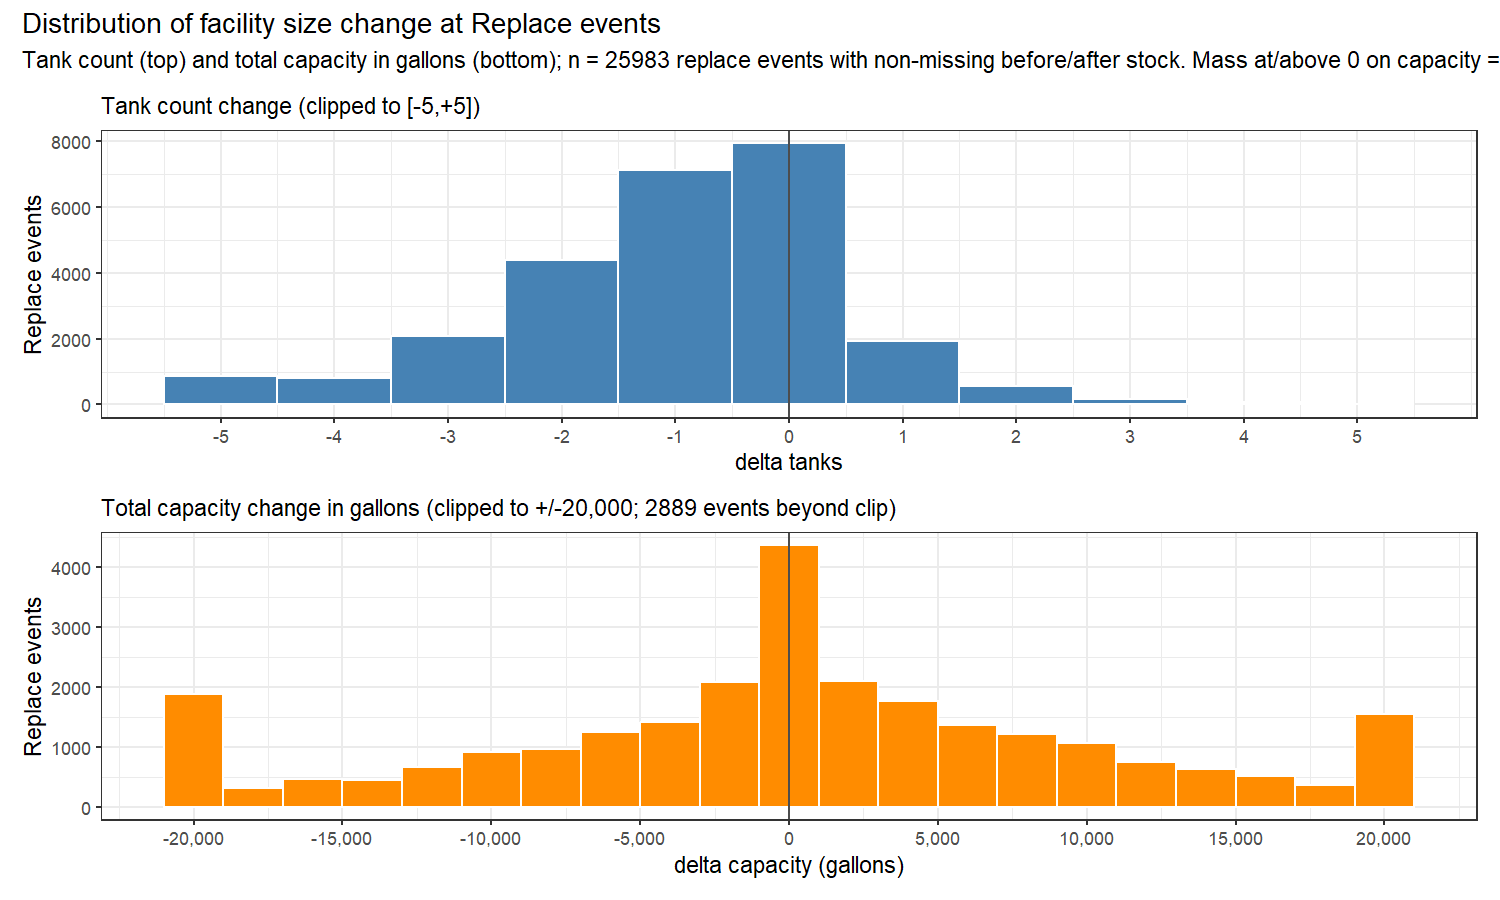
\includegraphics{../../Output/Figures/T011_A6_CapacityChange_Distribution.png}

}

\end{figure}%

\vspace{0.1cm}
\begin{flushleft}
\footnotesize
\textit{Notes:} Two-panel histogram of facility size change at Replace events: tank count (top, clipped to $[-5,+5]$) and total capacity in gallons (bottom, clipped to $\pm 20{,}000$; events beyond the clip are noted in the panel subtitle). Vertical line marks no change. The capacity distribution is roughly symmetric around zero, consistent with consolidation rather than systematic shrinkage.
\end{flushleft}

\subsubsection{Tank-count vs capacity change (joint)}\label{sec-t011-a7}

\begin{table}

\caption{\label{tbl-t011-a7}Tank-count change versus capacity change at
replace events}

\centering{

[!h]
\centering\begingroup\fontsize{8}{10}\selectfont

\resizebox{\ifdim\width>\linewidth\linewidth\else\width\fi}{!}{
\begin{tabular}{lrrrrrrr}
\toprule
Tank chg bin & N & Pct & Mean cap pct & Median cap pct & P25 cap pct & P75 cap pct & Pct cap-preserving\\
\midrule
<=-5 & 863 & 3.3214025 & 418.5309 & -48.27586 & -73.79863 & -19.56702 & 16.68598\\
-4 & 812 & 3.1251203 & 6615.0646 & -39.71983 & -71.39024 & -10.36391 & 24.87685\\
-3 & 2073 & 7.9782935 & 5526.7424 & -26.82927 & -52.38095 & -1.35635 & 32.94742\\
-2 & 4403 & 16.9456953 & 3323.1624 & -14.57859 & -40.00000 & 13.69022 & 45.78696\\
-1 & 7128 & 27.4333218 & 7164.9911 & 0.00000 & -25.00000 & 33.03769 & 61.64422\\
\addlinespace
0 & 7959 & 30.6315668 & 5383.8774 & 10.70111 & 0.00000 & 54.54545 & 84.57093\\
+1 & 1924 & 7.4048416 & 18929.9222 & 64.44612 & 25.00000 & 150.00000 & 95.21830\\
+2 & 568 & 2.1860447 & 33859.8252 & 132.57576 & 53.51190 & 353.01522 & 97.53521\\
+3 & 170 & 0.6542739 & 42317.1617 & 237.50000 & 88.91076 & 937.50000 & 99.41176\\
+4 & 61 & 0.2347689 & 61864.9945 & 336.95652 & 136.36364 & 950.00000 & 96.72131\\
\addlinespace
>=+5 & 22 & 0.0846707 & 2297.6946 & 527.14617 & 61.66047 & 2625.00000 & 100.00000\\
\bottomrule
\end{tabular}}
\endgroup{}

}

\end{table}%

\vspace{0.1cm}
\begin{flushleft}
\footnotesize
\textit{Notes:} Joint distribution of tank-count and capacity change at Replace events. For each tank-count-change bin: median and interquartile range of capacity percent change, and the share that is capacity-preserving (delta\_cap\_pct $\geq -10$). A negative tank-count bin with median capacity near zero is consolidation (fewer, larger tanks); a negative bin with strongly negative capacity is true shrinkage. The mean column is dominated by small-denominator outliers and is reported only for completeness; the figure plots the median.
\end{flushleft}

\subsubsection{Tank-count vs capacity change bin
scatter}\label{sec-t011-a7-fig}

\begin{figure}[H]

\caption{\label{fig-t011-a7}Tank-count change versus capacity change at
replace events (bin scatter)}

\centering{

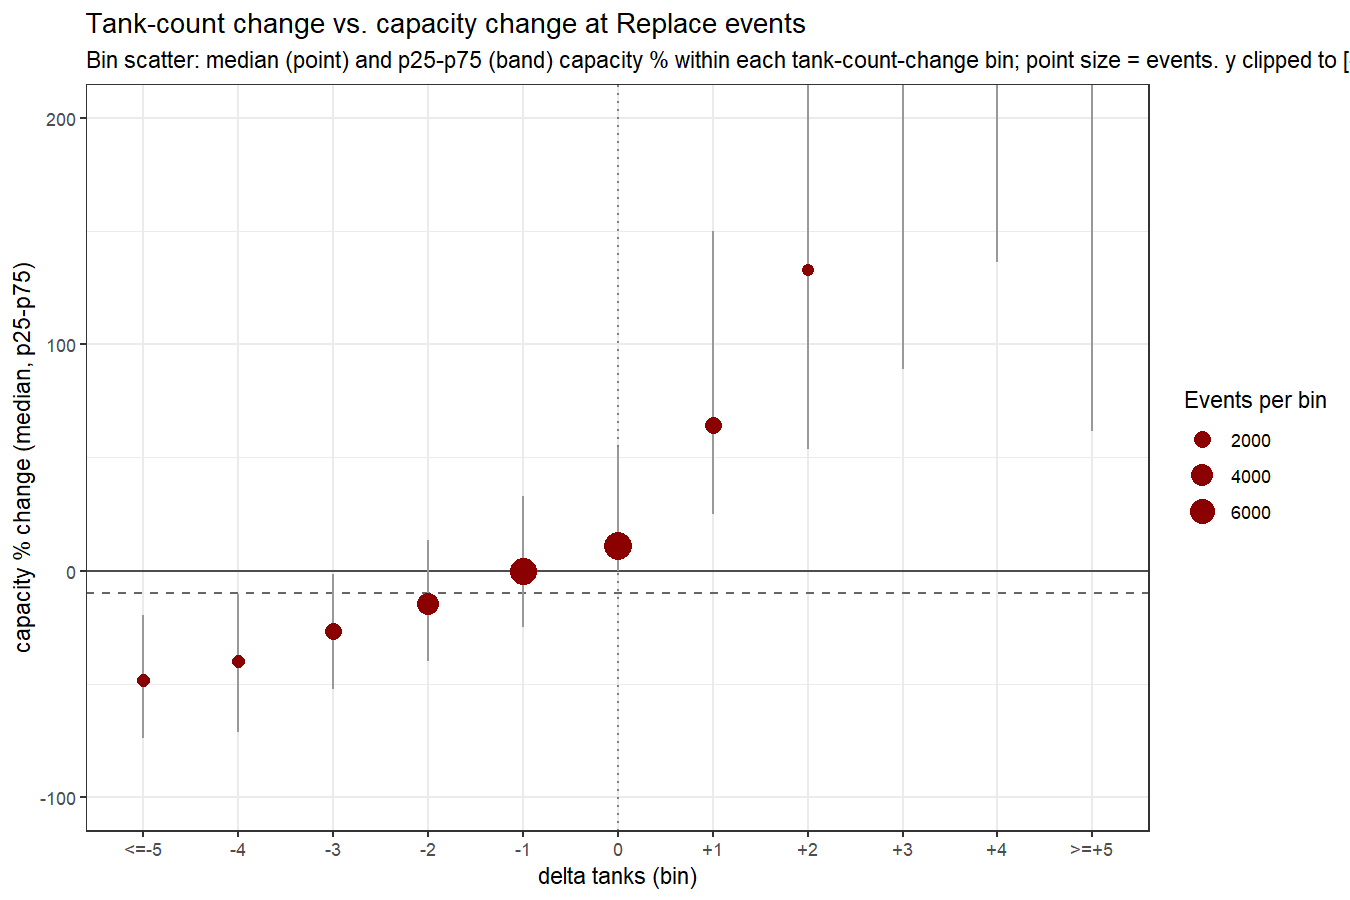
\includegraphics{../../Output/Figures/T011_A7_TankVsCapacity_BinScatter.png}

}

\end{figure}%

\vspace{0.1cm}
\begin{flushleft}
\footnotesize
\textit{Notes:} Bin scatter of capacity percent change against tank-count change at Replace events: median (point) and p25--p75 (band) within each tank-count-change bin; point area is the number of events. The y-axis is clipped to $[-100,+200]$ so the bands and reference lines are visible. Solid line at zero (capacity flat); dashed line at $-10$ (shrink threshold); dotted vertical line at zero tank change. Near zero capacity at negative tank change is consolidation; well below zero is true facility shrinkage.
\end{flushleft}

\subsection{Empirical CCPs by state cell}\label{sec-t011-ccp}

\subsubsection{Raw empirical CCP table --- all 32
cells}\label{sec-t011-b1}

\begin{table}

\caption{\label{tbl-t011-b1}Empirical choice probabilities by state
cell}

\centering{

[!h]
\centering\begingroup\fontsize{8}{10}\selectfont

\resizebox{\ifdim\width>\linewidth\linewidth\else\width\fi}{!}{
\begin{tabular}{rlllrrrrrrr}
\toprule
s & Age & Wall & Regime & N obs & P(M) & P(E) & P(R) & P(E|cl) & P(R|cl) & Cell pct\\
\midrule
1 & 0-5 & SW & FF & 46709 & 0.9833 & 0.01464 & 0.00201 & 0.879 & 0.121 & 2.05\\
2 & 5-10 & SW & FF & 97999 & 0.9852 & 0.01131 & 0.00350 & 0.764 & 0.236 & 4.29\\
3 & 10-15 & SW & FF & 180163 & 0.9749 & 0.02174 & 0.00340 & 0.865 & 0.135 & 7.89\\
4 & 15-20 & SW & FF & 240344 & 0.9715 & 0.02580 & 0.00271 & 0.905 & 0.095 & 10.53\\
5 & 20-25 & SW & FF & 255278 & 0.9719 & 0.02634 & 0.00174 & 0.938 & 0.062 & 11.18\\
\addlinespace
6 & 25-30 & SW & FF & 234030 & 0.9769 & 0.02198 & 0.00113 & 0.951 & 0.049 & 10.25\\
7 & 30-35 & SW & FF & 191377 & 0.9795 & 0.01953 & 0.00092 & 0.955 & 0.045 & 8.38\\
8 & 35+ & SW & FF & 410728 & 0.9852 & 0.01450 & 0.00032 & 0.978 & 0.022 & 17.99\\
9 & 0-5 & DW & FF & 64621 & 0.9990 & 0.00000 & 0.00099 & 0.000 & 1.000 & 2.83\\
10 & 5-10 & DW & FF & 77103 & 0.9936 & 0.00000 & 0.00636 & 0.000 & 1.000 & 3.38\\
\addlinespace
11 & 10-15 & DW & FF & 77966 & 0.9908 & 0.00000 & 0.00920 & 0.000 & 1.000 & 3.42\\
12 & 15-20 & DW & FF & 62241 & 0.9893 & 0.00000 & 0.01067 & 0.000 & 1.000 & 2.73\\
13 & 20-25 & DW & FF & 41520 & 0.9931 & 0.00000 & 0.00686 & 0.000 & 1.000 & 1.82\\
14 & 25-30 & DW & FF & 20407 & 0.9974 & 0.00000 & 0.00265 & 0.000 & 1.000 & 0.89\\
15 & 30-35 & DW & FF & 4872 & 0.9947 & 0.00000 & 0.00534 & 0.000 & 1.000 & 0.21\\
\addlinespace
16 & 35+ & DW & FF & 2867 & 0.9962 & 0.00000 & 0.00384 & 0.000 & 1.000 & 0.13\\
17 & 0-5 & SW & RB & 3350 & 0.9937 & 0.00537 & 0.00090 & 0.857 & 0.143 & 0.15\\
18 & 5-10 & SW & RB & 9999 & 0.9881 & 0.01120 & 0.00070 & 0.941 & 0.059 & 0.44\\
19 & 10-15 & SW & RB & 19093 & 0.9873 & 0.01042 & 0.00225 & 0.822 & 0.178 & 0.84\\
20 & 15-20 & SW & RB & 26212 & 0.9775 & 0.02056 & 0.00198 & 0.912 & 0.088 & 1.15\\
\addlinespace
21 & 20-25 & SW & RB & 36841 & 0.9727 & 0.02581 & 0.00149 & 0.945 & 0.055 & 1.61\\
22 & 25-30 & SW & RB & 37789 & 0.9732 & 0.02485 & 0.00198 & 0.926 & 0.074 & 1.66\\
23 & 30-35 & SW & RB & 31888 & 0.9685 & 0.02923 & 0.00223 & 0.929 & 0.071 & 1.40\\
24 & 35+ & SW & RB & 30722 & 0.9579 & 0.04007 & 0.00205 & 0.951 & 0.049 & 1.35\\
25 & 0-5 & DW & RB & 18813 & 0.9995 & 0.00000 & 0.00053 & 0.000 & 1.000 & 0.82\\
\addlinespace
26 & 5-10 & DW & RB & 16557 & 0.9943 & 0.00000 & 0.00568 & 0.000 & 1.000 & 0.73\\
27 & 10-15 & DW & RB & 14499 & 0.9926 & 0.00000 & 0.00738 & 0.000 & 1.000 & 0.64\\
28 & 15-20 & DW & RB & 13106 & 0.9802 & 0.00000 & 0.01976 & 0.000 & 1.000 & 0.57\\
29 & 20-25 & DW & RB & 8677 & 0.9749 & 0.00000 & 0.02512 & 0.000 & 1.000 & 0.38\\
30 & 25-30 & DW & RB & 4218 & 0.9829 & 0.00000 & 0.01707 & 0.000 & 1.000 & 0.18\\
\addlinespace
31 & 30-35 & DW & RB & 1770 & 0.9808 & 0.00000 & 0.01921 & 0.000 & 1.000 & 0.08\\
32 & 35+ & DW & RB & 976 & 0.9816 & 0.00000 & 0.01844 & 0.000 & 1.000 & 0.04\\
\bottomrule
\end{tabular}}
\endgroup{}

}

\end{table}%

\vspace{0.1cm}
\begin{flushleft}
\footnotesize
\textit{Notes:} Raw empirical choice probabilities by state cell (age $\times$ wall $\times$ regime; 32 cells). Wall: SW = single-walled, DW = double-walled. Regime: FF = flat-fee, RB = risk-based. P(M)$+$P(E)$+$P(R)$=1$ by construction; P(E$\mid$cl) and P(R$\mid$cl) are conditional on a closure and sum to 1. Every DW closure is coded Replace, so P(R$\mid$cl)$=1$ for all DW cells. Cell pct is the cell's share of the estimation sample; sparse cells should be read with caution.
\end{flushleft}

\subsubsection{Empirical CCPs --- single-walled
panel}\label{sec-t011-b1-sw}

\begin{figure}[H]

\caption{\label{fig-t011-b1-sw}Empirical choice probabilities,
single-walled facilities}

\centering{

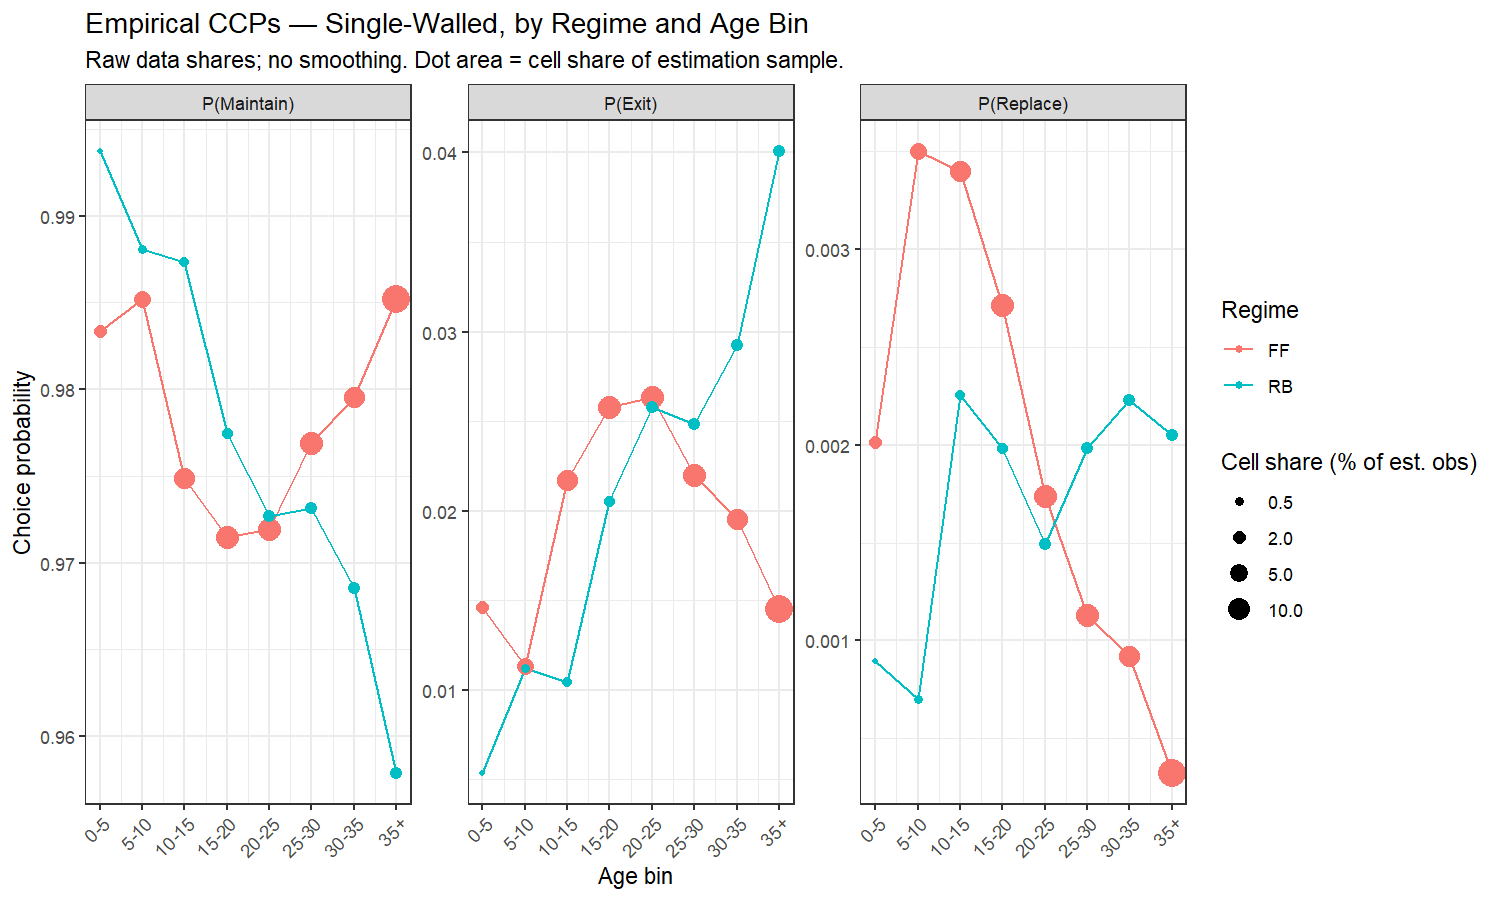
\includegraphics{../../Output/Figures/T011_B1_EmpiricalCCPs_SW.png}

}

\end{figure}%

\vspace{0.1cm}
\begin{flushleft}
\footnotesize
\textit{Notes:} Single-walled facilities. Raw data shares by age bin, faceted by action (Maintain, Exit, Replace); no smoothing. Dot area is the cell's share of the estimation sample. FF = flat-fee, RB = risk-based.
\end{flushleft}

\subsubsection{Empirical CCPs --- double-walled
panel}\label{sec-t011-b2-dw}

\begin{figure}[H]

\caption{\label{fig-t011-b2-dw}Empirical choice probabilities,
double-walled facilities}

\centering{

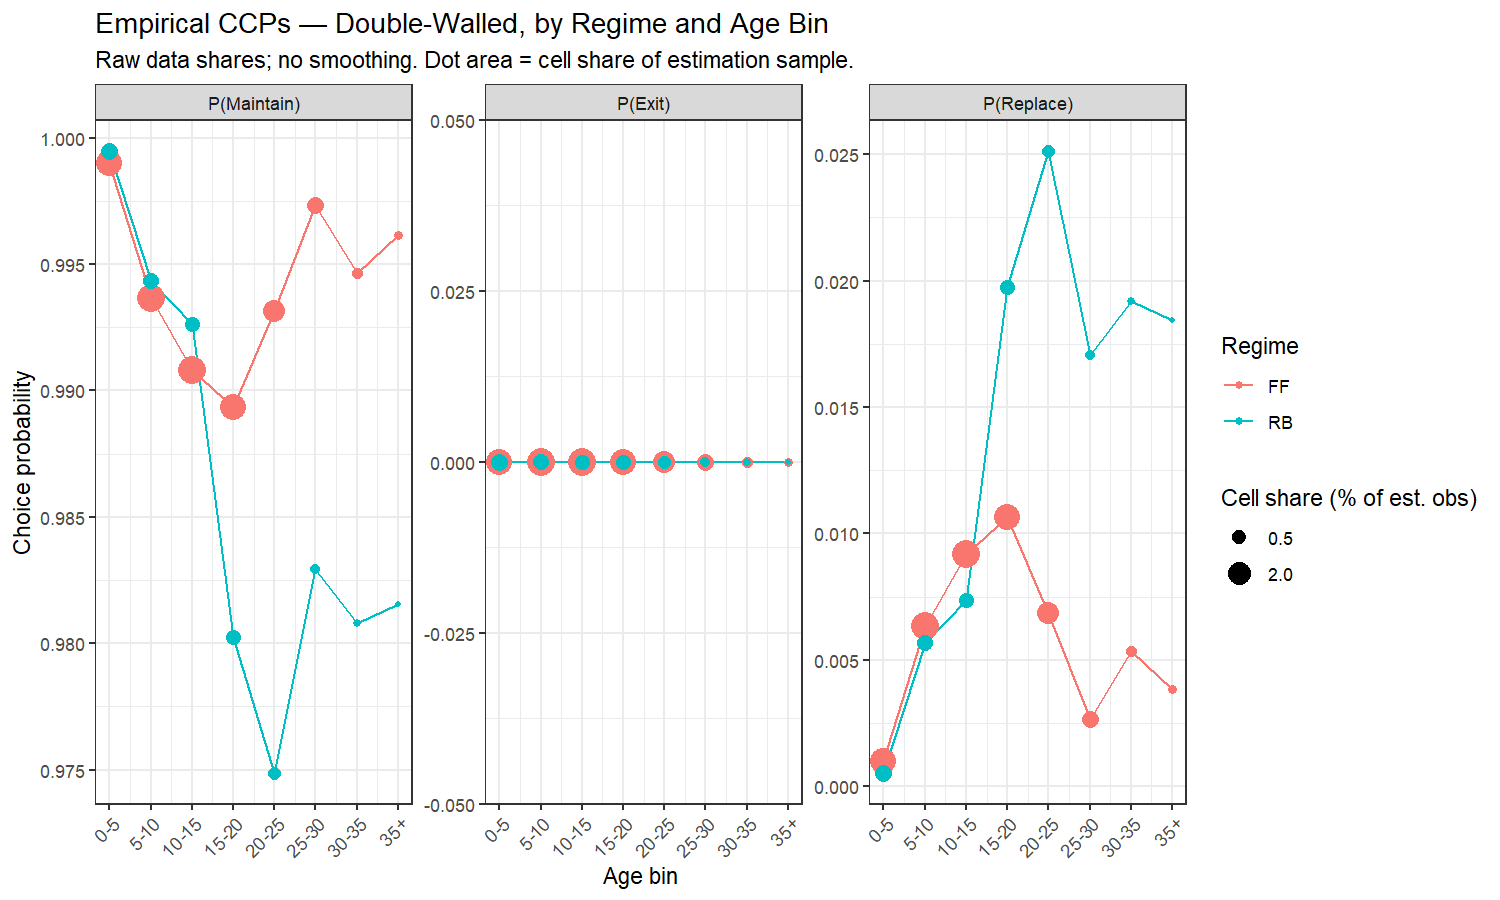
\includegraphics{../../Output/Figures/T011_B2_EmpiricalCCPs_DW.png}

}

\end{figure}%

\vspace{0.1cm}
\begin{flushleft}
\footnotesize
\textit{Notes:} Double-walled facilities. Raw data shares by age bin, faceted by action; no smoothing. Dot area is the cell's share of the estimation sample. Double-walled closures are coded Replace by construction, so the Exit panel is empty. FF = flat-fee, RB = risk-based.
\end{flushleft}

\subsubsection{P(Replace \textbar{} Closure) by age, wall, and
regime}\label{sec-t011-b3}

\begin{figure}[H]

\caption{\label{fig-t011-b3}Replace share among closures, by age, wall,
and regime}

\centering{

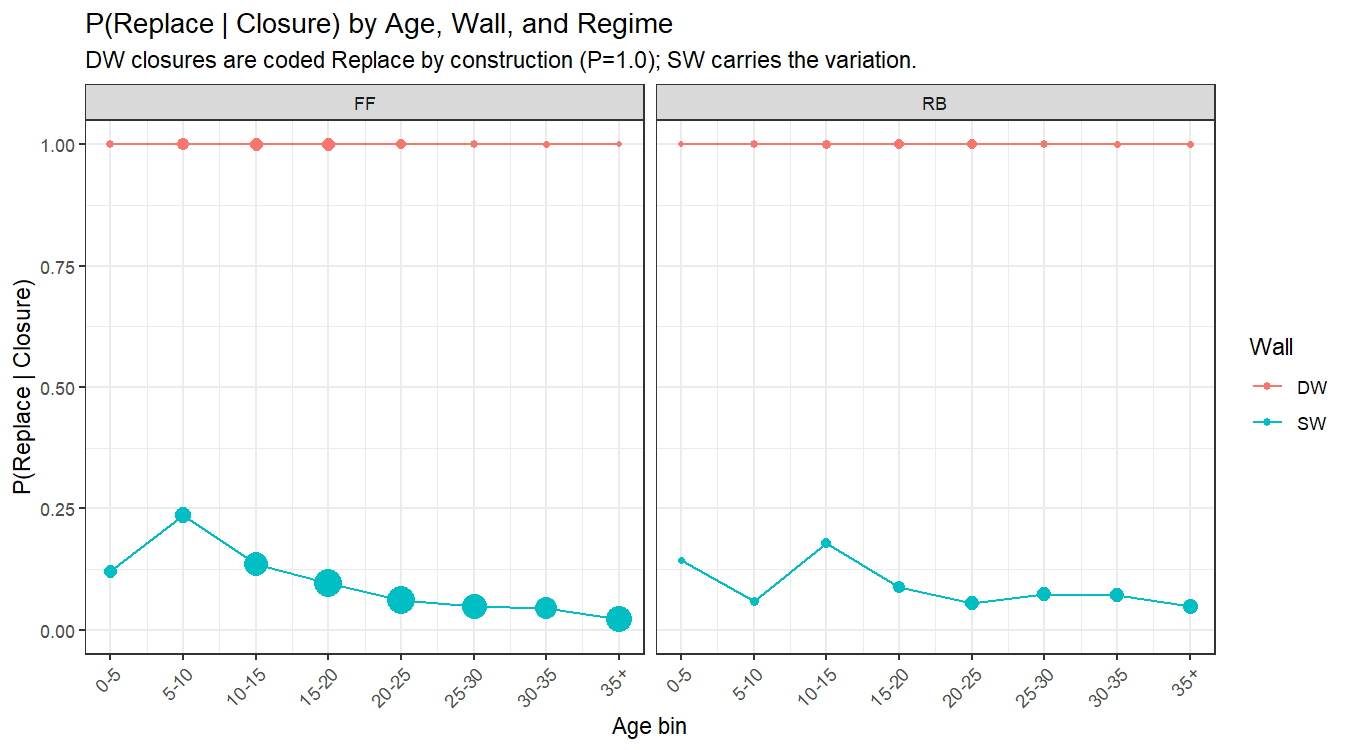
\includegraphics{../../Output/Figures/T011_B3_ReplaceShareAmongClosures.png}

}

\end{figure}%

\vspace{0.1cm}
\begin{flushleft}
\footnotesize
\textit{Notes:} Conditional replace share among closures, faceted by pricing regime (FF, RB) and colored by wall type. Double-walled closures are coded Replace by construction (P $=1.0$ in every cell), so the single-walled series carries all the identifying variation. Point area is the number of closures in the cell.
\end{flushleft}

\subsection{CCP variation by facility size}\label{sec-t011-size}

\subsubsection{CCPs by (size bin x state cell)}\label{sec-t011-c1}

\begingroup\fontsize{8}{10}\selectfont

\begin{longtable}{llllrrrrrr}

\caption{\label{tbl-t011-c1}Empirical choice probabilities by facility
size and state cell}

\tabularnewline

\toprule
Size & Age & Wall & Regime & N obs & P(M) & P(E) & P(R) & P(E|cl) & P(R|cl)\\
\midrule
\endfirsthead
\multicolumn{10}{@{}l}{\textit{(continued)}}\\
\toprule
Size & Age & Wall & Regime & N obs & P(M) & P(E) & P(R) & P(E|cl) & P(R|cl)\\
\midrule
\endhead

\endfoot
\bottomrule
\endlastfoot
1 & 0-5 & SW & FF & 9914 & 0.9572 & 0.03904 & 0.00373 & 0.913 & 0.087\\
1 & 5-10 & SW & FF & 19280 & 0.9702 & 0.02619 & 0.00363 & 0.878 & 0.122\\
1 & 10-15 & SW & FF & 33079 & 0.9487 & 0.04973 & 0.00160 & 0.969 & 0.031\\
1 & 15-20 & SW & FF & 43487 & 0.9506 & 0.04854 & 0.00090 & 0.982 & 0.018\\
1 & 20-25 & SW & FF & 48906 & 0.9530 & 0.04678 & 0.00022 & 0.995 & 0.005\\
\addlinespace
1 & 25-30 & SW & FF & 49233 & 0.9687 & 0.03110 & 0.00016 & 0.995 & 0.005\\
1 & 30-35 & SW & FF & 46427 & 0.9783 & 0.02158 & 0.00015 & 0.993 & 0.007\\
1 & 35+ & SW & FF & 146549 & 0.9868 & 0.01317 & 0.00004 & 0.997 & 0.003\\
1 & 0-5 & DW & FF & 12009 & 0.9984 & 0.00000 & 0.00158 & 0.000 & 1.000\\
1 & 5-10 & DW & FF & 17907 & 0.9953 & 0.00000 & 0.00469 & 0.000 & 1.000\\
\addlinespace
1 & 10-15 & DW & FF & 20331 & 0.9978 & 0.00000 & 0.00221 & 0.000 & 1.000\\
1 & 15-20 & DW & FF & 17177 & 0.9990 & 0.00000 & 0.00105 & 0.000 & 1.000\\
1 & 20-25 & DW & FF & 12403 & 0.9999 & 0.00000 & 0.00008 & 0.000 & 1.000\\
1 & 25-30 & DW & FF & 6584 & 1.0000 & 0.00000 & 0.00000 & 0.000 & 0.000\\
1 & 30-35 & DW & FF & 1468 & 1.0000 & 0.00000 & 0.00000 & 0.000 & 0.000\\
\addlinespace
1 & 35+ & DW & FF & 1083 & 1.0000 & 0.00000 & 0.00000 & 0.000 & 0.000\\
1 & 0-5 & SW & RB & 1113 & 0.9919 & 0.00629 & 0.00180 & 0.778 & 0.222\\
1 & 5-10 & SW & RB & 3059 & 0.9853 & 0.01471 & 0.00000 & 1.000 & 0.000\\
1 & 10-15 & SW & RB & 5029 & 0.9879 & 0.01133 & 0.00080 & 0.934 & 0.066\\
1 & 15-20 & SW & RB & 5123 & 0.9588 & 0.04060 & 0.00059 & 0.986 & 0.014\\
\addlinespace
1 & 20-25 & SW & RB & 4360 & 0.9365 & 0.06353 & 0.00000 & 1.000 & 0.000\\
1 & 25-30 & SW & RB & 2896 & 0.9275 & 0.07251 & 0.00000 & 1.000 & 0.000\\
1 & 30-35 & SW & RB & 2183 & 0.9290 & 0.07055 & 0.00046 & 0.994 & 0.006\\
1 & 35+ & SW & RB & 2597 & 0.9322 & 0.06700 & 0.00077 & 0.989 & 0.011\\
1 & 0-5 & DW & RB & 4786 & 0.9990 & 0.00000 & 0.00104 & 0.000 & 1.000\\
\addlinespace
1 & 5-10 & DW & RB & 3769 & 0.9966 & 0.00000 & 0.00345 & 0.000 & 1.000\\
1 & 10-15 & DW & RB & 3278 & 0.9991 & 0.00000 & 0.00092 & 0.000 & 1.000\\
1 & 15-20 & DW & RB & 2942 & 0.9993 & 0.00000 & 0.00068 & 0.000 & 1.000\\
1 & 20-25 & DW & RB & 1861 & 0.9995 & 0.00000 & 0.00054 & 0.000 & 1.000\\
1 & 25-30 & DW & RB & 797 & 1.0000 & 0.00000 & 0.00000 & 0.000 & 0.000\\
\addlinespace
1 & 30-35 & DW & RB & 242 & 1.0000 & 0.00000 & 0.00000 & 0.000 & 0.000\\
1 & 35+ & DW & RB & 78 & 1.0000 & 0.00000 & 0.00000 & 0.000 & 0.000\\
2 & 0-5 & SW & FF & 16757 & 0.9879 & 0.01068 & 0.00143 & 0.882 & 0.118\\
2 & 5-10 & SW & FF & 31727 & 0.9877 & 0.00987 & 0.00246 & 0.801 & 0.199\\
2 & 10-15 & SW & FF & 45930 & 0.9742 & 0.02297 & 0.00285 & 0.890 & 0.110\\
\addlinespace
2 & 15-20 & SW & FF & 53940 & 0.9694 & 0.02937 & 0.00128 & 0.958 & 0.042\\
2 & 20-25 & SW & FF & 53894 & 0.9695 & 0.02954 & 0.00095 & 0.969 & 0.031\\
2 & 25-30 & SW & FF & 46106 & 0.9754 & 0.02410 & 0.00048 & 0.981 & 0.019\\
2 & 30-35 & SW & FF & 38146 & 0.9787 & 0.02087 & 0.00039 & 0.982 & 0.018\\
2 & 35+ & SW & FF & 97096 & 0.9838 & 0.01597 & 0.00022 & 0.987 & 0.013\\
\addlinespace
2 & 0-5 & DW & FF & 23515 & 0.9991 & 0.00000 & 0.00085 & 0.000 & 1.000\\
2 & 5-10 & DW & FF & 25952 & 0.9964 & 0.00000 & 0.00362 & 0.000 & 1.000\\
2 & 10-15 & DW & FF & 23585 & 0.9958 & 0.00000 & 0.00424 & 0.000 & 1.000\\
2 & 15-20 & DW & FF & 17922 & 0.9967 & 0.00000 & 0.00335 & 0.000 & 1.000\\
2 & 20-25 & DW & FF & 10741 & 0.9980 & 0.00000 & 0.00196 & 0.000 & 1.000\\
\addlinespace
2 & 25-30 & DW & FF & 4352 & 0.9986 & 0.00000 & 0.00138 & 0.000 & 1.000\\
2 & 30-35 & DW & FF & 951 & 0.9989 & 0.00000 & 0.00105 & 0.000 & 1.000\\
2 & 35+ & DW & FF & 548 & 0.9964 & 0.00000 & 0.00365 & 0.000 & 1.000\\
2 & 0-5 & SW & RB & 1884 & 0.9942 & 0.00531 & 0.00053 & 0.909 & 0.091\\
2 & 5-10 & SW & RB & 5426 & 0.9891 & 0.01032 & 0.00055 & 0.949 & 0.051\\
\addlinespace
2 & 10-15 & SW & RB & 9565 & 0.9895 & 0.01004 & 0.00042 & 0.960 & 0.040\\
2 & 15-20 & SW & RB & 10207 & 0.9823 & 0.01656 & 0.00118 & 0.934 & 0.066\\
2 & 20-25 & SW & RB & 8980 & 0.9748 & 0.02416 & 0.00100 & 0.960 & 0.040\\
2 & 25-30 & SW & RB & 6680 & 0.9651 & 0.03353 & 0.00135 & 0.961 & 0.039\\
2 & 30-35 & SW & RB & 5552 & 0.9557 & 0.04359 & 0.00072 & 0.984 & 0.016\\
\addlinespace
2 & 35+ & SW & RB & 6884 & 0.9542 & 0.04503 & 0.00073 & 0.984 & 0.016\\
2 & 0-5 & DW & RB & 9926 & 0.9997 & 0.00000 & 0.00030 & 0.000 & 1.000\\
2 & 5-10 & DW & RB & 8611 & 0.9931 & 0.00000 & 0.00685 & 0.000 & 1.000\\
2 & 10-15 & DW & RB & 6826 & 0.9963 & 0.00000 & 0.00366 & 0.000 & 1.000\\
2 & 15-20 & DW & RB & 5368 & 0.9933 & 0.00000 & 0.00671 & 0.000 & 1.000\\
\addlinespace
2 & 20-25 & DW & RB & 2763 & 0.9949 & 0.00000 & 0.00507 & 0.000 & 1.000\\
2 & 25-30 & DW & RB & 900 & 0.9900 & 0.00000 & 0.01000 & 0.000 & 1.000\\
2 & 30-35 & DW & RB & 300 & 0.9900 & 0.00000 & 0.01000 & 0.000 & 1.000\\
2 & 35+ & DW & RB & 204 & 0.9951 & 0.00000 & 0.00490 & 0.000 & 1.000\\
3 & 0-5 & SW & FF & 11875 & 0.9936 & 0.00514 & 0.00126 & 0.803 & 0.197\\
\addlinespace
3 & 5-10 & SW & FF & 26390 & 0.9892 & 0.00765 & 0.00311 & 0.711 & 0.289\\
3 & 10-15 & SW & FF & 50962 & 0.9826 & 0.01430 & 0.00306 & 0.824 & 0.176\\
3 & 15-20 & SW & FF & 68760 & 0.9765 & 0.02065 & 0.00282 & 0.880 & 0.120\\
3 & 20-25 & SW & FF & 73388 & 0.9773 & 0.02122 & 0.00153 & 0.933 & 0.067\\
3 & 25-30 & SW & FF & 66403 & 0.9780 & 0.02084 & 0.00111 & 0.949 & 0.051\\
\addlinespace
3 & 30-35 & SW & FF & 51189 & 0.9773 & 0.02163 & 0.00109 & 0.952 & 0.048\\
3 & 35+ & SW & FF & 80688 & 0.9838 & 0.01574 & 0.00051 & 0.969 & 0.031\\
3 & 0-5 & DW & FF & 18194 & 0.9992 & 0.00000 & 0.00077 & 0.000 & 1.000\\
3 & 5-10 & DW & FF & 21200 & 0.9915 & 0.00000 & 0.00854 & 0.000 & 1.000\\
3 & 10-15 & DW & FF & 20762 & 0.9858 & 0.00000 & 0.01421 & 0.000 & 1.000\\
\addlinespace
3 & 15-20 & DW & FF & 16356 & 0.9806 & 0.00000 & 0.01938 & 0.000 & 1.000\\
3 & 20-25 & DW & FF & 10729 & 0.9897 & 0.00000 & 0.01025 & 0.000 & 1.000\\
3 & 25-30 & DW & FF & 5256 & 0.9952 & 0.00000 & 0.00476 & 0.000 & 1.000\\
3 & 30-35 & DW & FF & 1307 & 0.9939 & 0.00000 & 0.00612 & 0.000 & 1.000\\
3 & 35+ & DW & FF & 511 & 0.9980 & 0.00000 & 0.00196 & 0.000 & 1.000\\
\addlinespace
3 & 0-5 & SW & RB & 261 & 0.9962 & 0.00383 & 0.00000 & 1.000 & 0.000\\
3 & 5-10 & SW & RB & 1147 & 0.9887 & 0.00785 & 0.00349 & 0.692 & 0.308\\
3 & 10-15 & SW & RB & 3342 & 0.9832 & 0.01137 & 0.00539 & 0.679 & 0.321\\
3 & 15-20 & SW & RB & 7333 & 0.9802 & 0.01677 & 0.00300 & 0.848 & 0.152\\
3 & 20-25 & SW & RB & 14372 & 0.9787 & 0.01969 & 0.00160 & 0.925 & 0.075\\
\addlinespace
3 & 25-30 & SW & RB & 17048 & 0.9791 & 0.01918 & 0.00176 & 0.916 & 0.084\\
3 & 30-35 & SW & RB & 14768 & 0.9772 & 0.02038 & 0.00237 & 0.896 & 0.104\\
3 & 35+ & SW & RB & 13688 & 0.9630 & 0.03404 & 0.00292 & 0.921 & 0.079\\
3 & 0-5 & DW & RB & 2611 & 0.9996 & 0.00000 & 0.00038 & 0.000 & 1.000\\
3 & 5-10 & DW & RB & 3101 & 0.9932 & 0.00000 & 0.00677 & 0.000 & 1.000\\
\addlinespace
3 & 10-15 & DW & RB & 3442 & 0.9855 & 0.00000 & 0.01453 & 0.000 & 1.000\\
3 & 15-20 & DW & RB & 3740 & 0.9607 & 0.00000 & 0.03930 & 0.000 & 1.000\\
3 & 20-25 & DW & RB & 2998 & 0.9613 & 0.00000 & 0.03869 & 0.000 & 1.000\\
3 & 25-30 & DW & RB & 1705 & 0.9789 & 0.00000 & 0.02111 & 0.000 & 1.000\\
3 & 30-35 & DW & RB & 848 & 0.9800 & 0.00000 & 0.02005 & 0.000 & 1.000\\
\addlinespace
3 & 35+ & DW & RB & 501 & 0.9900 & 0.00000 & 0.00998 & 0.000 & 1.000\\
4+ & 0-5 & SW & FF & 7887 & 0.9938 & 0.00431 & 0.00190 & 0.694 & 0.306\\
4+ & 5-10 & SW & FF & 20602 & 0.9902 & 0.00427 & 0.00548 & 0.438 & 0.562\\
4+ & 10-15 & SW & FF & 50192 & 0.9849 & 0.00970 & 0.00542 & 0.642 & 0.358\\
4+ & 15-20 & SW & FF & 74157 & 0.9806 & 0.01466 & 0.00472 & 0.756 & 0.244\\
\addlinespace
4+ & 20-25 & SW & FF & 79090 & 0.9803 & 0.01627 & 0.00341 & 0.827 & 0.173\\
4+ & 25-30 & SW & FF & 72288 & 0.9823 & 0.01548 & 0.00221 & 0.875 & 0.125\\
4+ & 30-35 & SW & FF & 55615 & 0.9833 & 0.01498 & 0.00176 & 0.895 & 0.105\\
4+ & 35+ & SW & FF & 86395 & 0.9853 & 0.01392 & 0.00075 & 0.949 & 0.051\\
4+ & 0-5 & DW & FF & 10438 & 0.9989 & 0.00000 & 0.00105 & 0.000 & 1.000\\
\addlinespace
4+ & 5-10 & DW & FF & 12044 & 0.9891 & 0.00000 & 0.01088 & 0.000 & 1.000\\
4+ & 10-15 & DW & FF & 13288 & 0.9792 & 0.00000 & 0.02085 & 0.000 & 1.000\\
4+ & 15-20 & DW & FF & 10786 & 0.9751 & 0.00000 & 0.02494 & 0.000 & 1.000\\
4+ & 20-25 & DW & FF & 7647 & 0.9800 & 0.00000 & 0.02001 & 0.000 & 1.000\\
4+ & 25-30 & DW & FF & 4215 & 0.9945 & 0.00000 & 0.00546 & 0.000 & 1.000\\
\addlinespace
4+ & 30-35 & DW & FF & 1146 & 0.9852 & 0.00000 & 0.01483 & 0.000 & 1.000\\
4+ & 35+ & DW & FF & 725 & 0.9890 & 0.00000 & 0.01103 & 0.000 & 1.000\\
4+ & 0-5 & SW & RB & 80 & 1.0000 & 0.00000 & 0.00000 & 0.000 & 0.000\\
4+ & 5-10 & SW & RB & 367 & 0.9946 & 0.00545 & 0.00000 & 1.000 & 0.000\\
4+ & 10-15 & SW & RB & 1157 & 0.9784 & 0.00691 & 0.01469 & 0.320 & 0.680\\
\addlinespace
4+ & 15-20 & SW & RB & 3549 & 0.9848 & 0.01099 & 0.00423 & 0.722 & 0.278\\
4+ & 20-25 & SW & RB & 9129 & 0.9784 & 0.01906 & 0.00252 & 0.883 & 0.117\\
4+ & 25-30 & SW & RB & 11165 & 0.9808 & 0.01594 & 0.00322 & 0.832 & 0.168\\
4+ & 30-35 & SW & RB & 9385 & 0.9717 & 0.02504 & 0.00330 & 0.883 & 0.117\\
4+ & 35+ & SW & RB & 7553 & 0.9607 & 0.03720 & 0.00212 & 0.946 & 0.054\\
\addlinespace
4+ & 0-5 & DW & RB & 1376 & 0.9993 & 0.00000 & 0.00073 & 0.000 & 1.000\\
4+ & 5-10 & DW & RB & 1076 & 0.9991 & 0.00000 & 0.00093 & 0.000 & 1.000\\
4+ & 10-15 & DW & RB & 953 & 0.9696 & 0.00000 & 0.03043 & 0.000 & 1.000\\
4+ & 15-20 & DW & RB & 1056 & 0.9299 & 0.00000 & 0.07008 & 0.000 & 1.000\\
4+ & 20-25 & DW & RB & 1055 & 0.9175 & 0.00000 & 0.08246 & 0.000 & 1.000\\
\addlinespace
4+ & 25-30 & DW & RB & 816 & 0.9669 & 0.00000 & 0.03309 & 0.000 & 1.000\\
4+ & 30-35 & DW & RB & 380 & 0.9632 & 0.00000 & 0.03684 & 0.000 & 1.000\\
4+ & 35+ & DW & RB & 193 & 0.9378 & 0.00000 & 0.06218 & 0.000 & 1.000\\
unknown & 0-5 & SW & FF & 276 & 0.9058 & 0.08333 & 0.01087 & 0.885 & 0.115\\
unknown & 0-5 & DW & FF & 465 & 1.0000 & 0.00000 & 0.00000 & 0.000 & 0.000\\
\addlinespace
unknown & 0-5 & DW & RB & 114 & 1.0000 & 0.00000 & 0.00000 & 0.000 & 0.000\\*

\end{longtable}

\endgroup{}

\vspace{0.1cm}
\begin{flushleft}
\footnotesize
\textit{Notes:} Empirical CCPs by (size bin $\times$ state cell); cells with fewer than 20 observations excluded. Facility size is the beginning-of-year tank count (Section 1.5). P(E$\mid$cl) and P(R$\mid$cl) are conditional on a closure. If the conditional shares are roughly constant across size bins within the same (age, wall, regime) cell, facility size does not belong in the DCM state space.
\end{flushleft}

\subsubsection{Exit rate by size x age (SW)}\label{sec-t011-c1-fig}

\begin{figure}[H]

\caption{\label{fig-t011-c1}Exit rate by facility size and age
(single-walled)}

\centering{

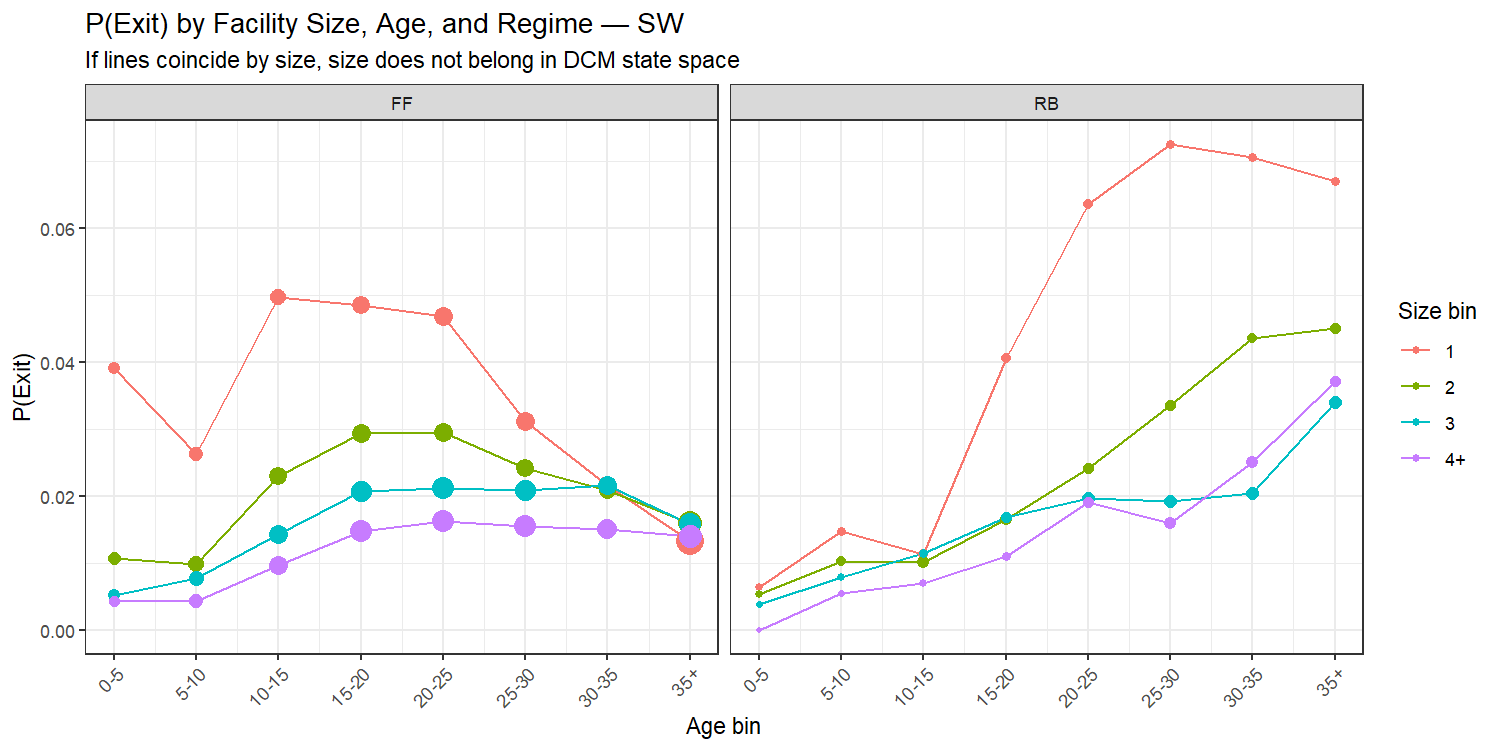
\includegraphics{../../Output/Figures/T011_C1_ExitRate_by_Size_SW.png}

}

\end{figure}%

\vspace{0.1cm}
\begin{flushleft}
\footnotesize
\textit{Notes:} Exit rate by facility size, age, and regime, single-walled facilities only; cells with fewer than 20 observations dropped. Four lines correspond to the four beginning-of-year size bins. Coincident lines imply facility size does not belong in the DCM state space.
\end{flushleft}

\subsubsection{Replace rate by size x age (SW)}\label{sec-t011-c2-fig}

\begin{figure}[H]

\caption{\label{fig-t011-c2}Replace rate by facility size and age
(single-walled)}

\centering{

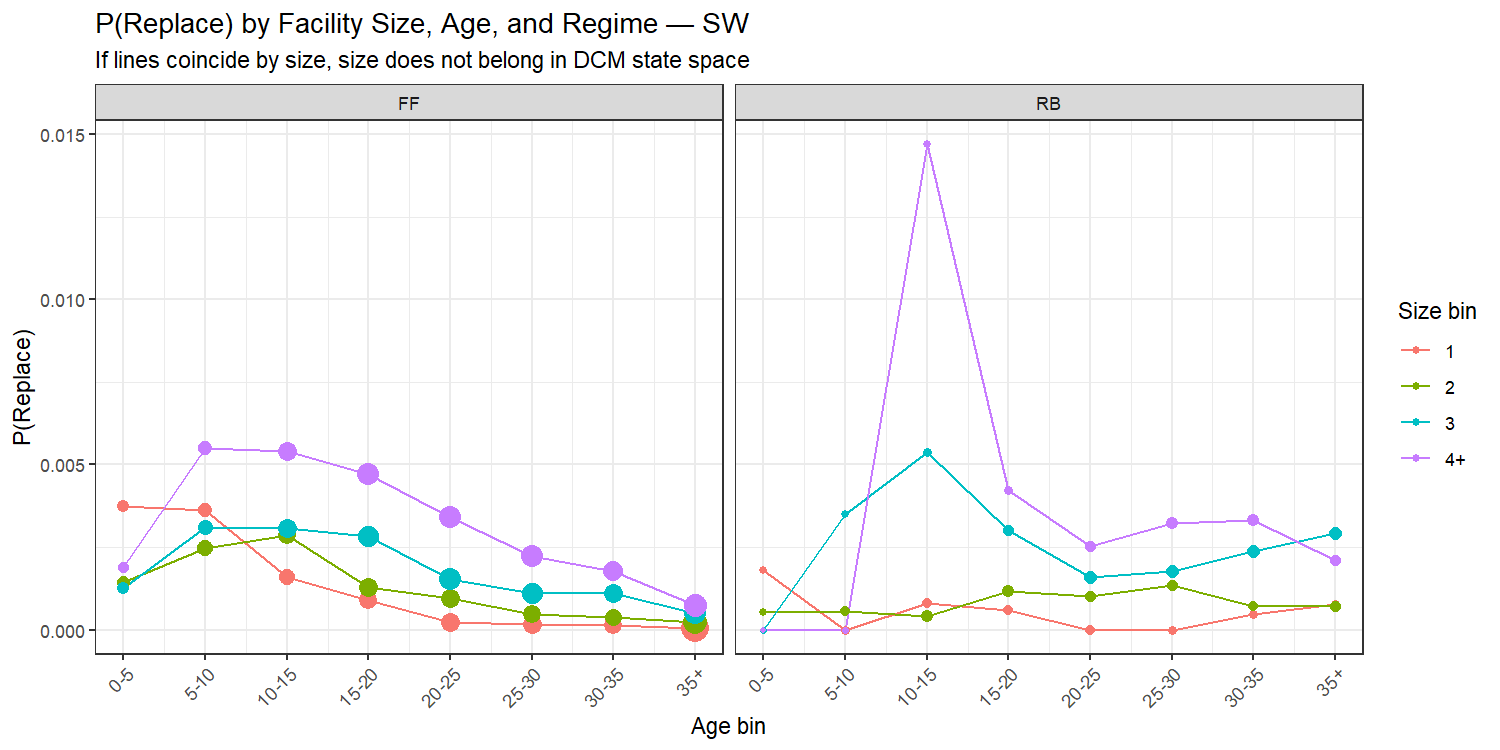
\includegraphics{../../Output/Figures/T011_C2_ReplaceRate_by_Size_SW.png}

}

\end{figure}%

\vspace{0.1cm}
\begin{flushleft}
\footnotesize
\textit{Notes:} Replace rate by facility size, age, and regime, single-walled facilities only; cells with fewer than 20 observations dropped. Four lines correspond to the four beginning-of-year size bins. Coincident lines imply facility size does not belong in the DCM state space.
\end{flushleft}

\subsubsection{Partial closure composition by size and
regime}\label{sec-t011-c2}

\begin{table}

\caption{\label{tbl-t011-c2}Closure composition by facility size and
pricing regime}

\centering{

[!h]
\centering\begingroup\fontsize{9}{11}\selectfont

\resizebox{\ifdim\width>\linewidth\linewidth\else\width\fi}{!}{
\begin{tabular}{llrrrrrrr}
\toprule
Size & Regime & N events & N partial & N full exit & N full replace & Pct partial & Pct exit & Pct replace\\
\midrule
1 & Control\_FF & 55774 & 2739 & 52189 & 846 & 4.9 & 93.6 & 1.5\\
1 & TX\_FF & 13039 & 375 & 12514 & 150 & 2.9 & 96.0 & 1.2\\
1 & TX\_RB & 2453 & 56 & 2377 & 20 & 2.3 & 96.9 & 0.8\\
2 & Control\_FF & 42909 & 9029 & 33023 & 857 & 21.0 & 77.0 & 2.0\\
2 & TX\_FF & 9998 & 1239 & 8579 & 180 & 12.4 & 85.8 & 1.8\\
\addlinespace
2 & TX\_RB & 2825 & 378 & 2379 & 68 & 13.4 & 84.2 & 2.4\\
3 & Control\_FF & 35826 & 11810 & 22880 & 1136 & 33.0 & 63.9 & 3.2\\
3 & TX\_FF & 8203 & 1946 & 5918 & 339 & 23.7 & 72.1 & 4.1\\
3 & TX\_RB & 4117 & 993 & 2882 & 242 & 24.1 & 70.0 & 5.9\\
4+ & Control\_FF & 47737 & 27157 & 19180 & 1400 & 56.9 & 40.2 & 2.9\\
\addlinespace
4+ & TX\_FF & 9276 & 4310 & 4614 & 352 & 46.5 & 49.7 & 3.8\\
4+ & TX\_RB & 3036 & 1101 & 1793 & 142 & 36.3 & 59.1 & 4.7\\
\bottomrule
\end{tabular}}
\endgroup{}

}

\end{table}%

\vspace{0.1cm}
\begin{flushleft}
\footnotesize
\textit{Notes:} Closure composition among facility-years with at least one closure, by beginning-of-year size bin and pricing regime, from the full facility panel (not restricted to the DCM estimation sample). Pct partial = portfolio shrinkage (some tanks closed, facility survives); pct full exit = complete walk-away with no future install; pct full replace = complete closure with a future install. The three shares sum to 100 within each row.
\end{flushleft}

\subsubsection{Closure composition stacked bar}\label{sec-t011-c3-fig}

\begin{figure}[H]

\caption{\label{fig-t011-c3}Closure composition by facility size and
regime}

\centering{

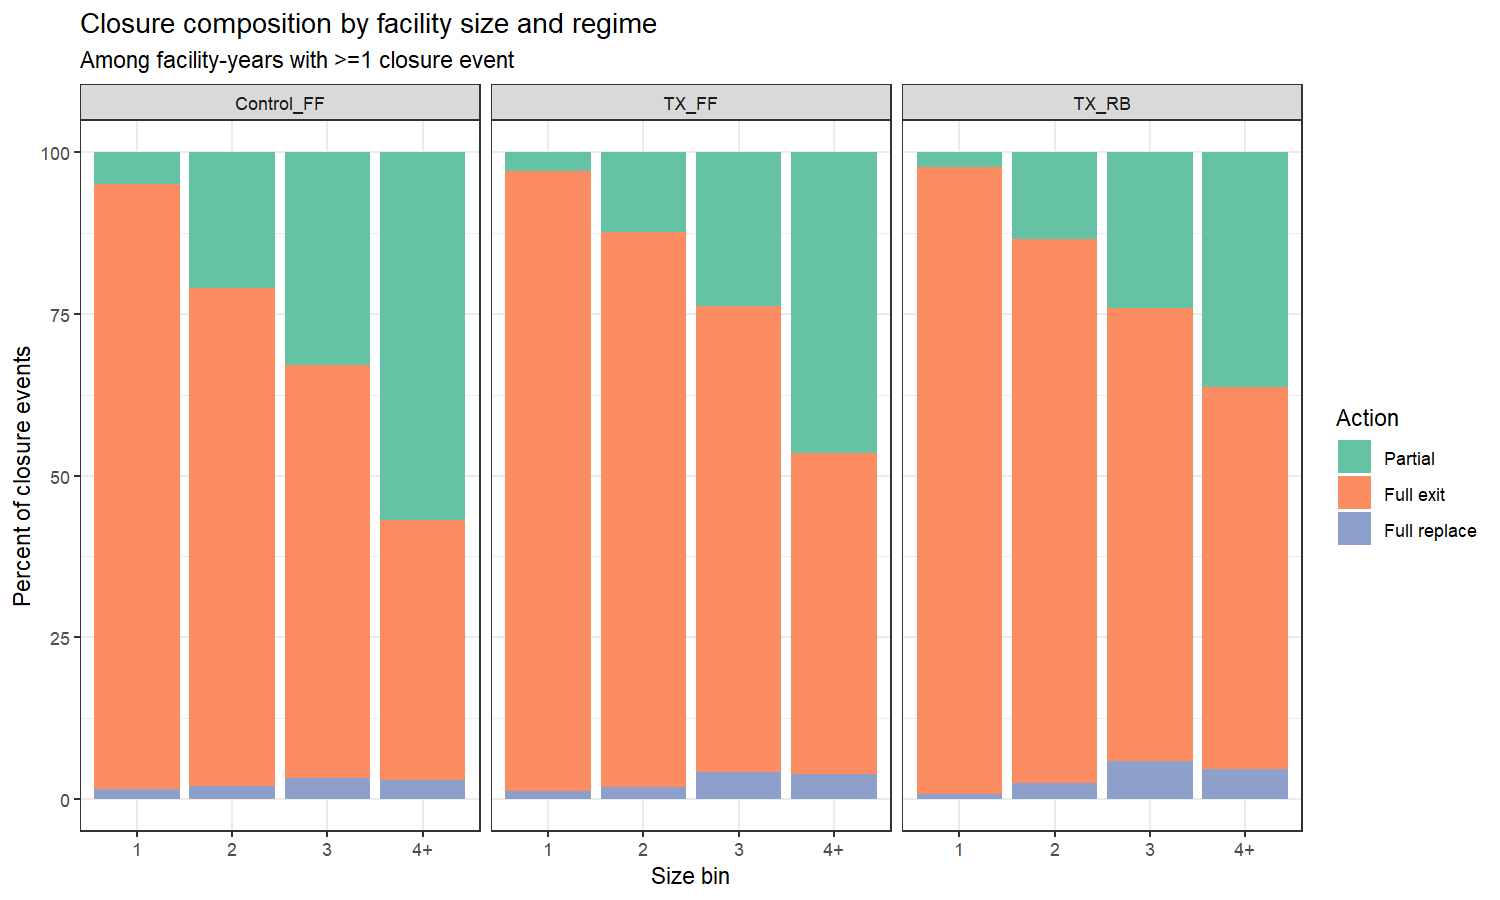
\includegraphics{../../Output/Figures/T011_C3_ClosureComposition_by_Size.png}

}

\end{figure}%

\vspace{0.1cm}
\begin{flushleft}
\footnotesize
\textit{Notes:} Closure composition (partial, full exit, full replace) by beginning-of-year facility size and regime, among facility-years with at least one closure. Bars are shown only for size $\times$ regime cells with at least 30 closure events. Partial closures rise steeply with facility size.
\end{flushleft}



\end{document}
